\documentclass[11pt,letterpaper]{article}
\usepackage[T1]{fontenc}
\usepackage{lmodern,microtype}
\usepackage[margin=1in,headheight=15pt]{geometry}
\usepackage{amsmath,amssymb,amsthm,mathtools}
\usepackage{booktabs,longtable,array,enumitem,graphicx,xcolor}
\usepackage{listings,fancyhdr}
\newcolumntype{P}[1]{>{\raggedright\arraybackslash}p{#1}}
\usepackage[colorlinks=true,linkcolor=teal!65!black,citecolor=teal!65!black,
 urlcolor=blue!55!black,breaklinks=true]{hyperref}
\usepackage[nameinlink,noabbrev]{cleveref}
\definecolor{ink}{RGB}{24,42,60}
\definecolor{accent}{RGB}{16,105,112}
\newcommand{\poly}{\operatorname{poly}}
\newcommand{\rk}{\operatorname{rk}}
\newcommand{\pin}{\texttt{c6d0ec8aa0b6308310ab6c081ba29d8bc363ede5}}
\newcommand{\code}[1]{\texttt{\detokenize{#1}}}
\newtheorem{theorem}{Theorem}[section]
\newtheorem{lemma}[theorem]{Lemma}
\newtheorem{proposition}[theorem]{Proposition}
\newtheorem{corollary}[theorem]{Corollary}
\theoremstyle{definition}
\newtheorem{definition}[theorem]{Definition}
\newtheorem{example}[theorem]{Example}
\theoremstyle{remark}
\newtheorem{remark}[theorem]{Remark}
\numberwithin{equation}{section}
\setlist{itemsep=3pt,topsep=6pt}
\setlength{\emergencystretch}{2em}
\lstset{basicstyle=\ttfamily\footnotesize,breaklines=true,columns=fullflexible,
 keepspaces=true,frame=single,rulecolor=\color{black!15},
 backgroundcolor=\color{black!2},showstringspaces=false}
\pagestyle{fancy}
\fancyhf{}
\fancyhead[L]{\small\color{ink}Exceptional rows and certificate replay}
\fancyhead[R]{\small ProveIt research}
\fancyfoot[C]{\thepage}
\hypersetup{pdftitle={Exceptional Rows and Fast Certificate Replay for Unknot Recognition},
 pdfauthor={ProveIt research continuation},
 pdfsubject={Parameterized forest selection, Boolean determinant sieving, and verified interval contraction}}

\begin{document}
\hypersetup{pageanchor=false}
\begin{titlepage}
\setlength{\parindent}{0pt}
\vspace*{0.1in}
{\color{accent}\large TOPOLOGY / ALGORITHMS / VERIFIED COMPUTATION\par}
\vspace{0.20in}
{\color{ink}\Huge\bfseries Exceptional Rows and\\Fast Certificate Replay\par}
\vspace{0.18in}
{\color{ink}\LARGE for Unknot Recognition\par}
\vspace{0.18in}
{\large Exact forest selection, a Boolean determinant sieve,\par
and authenticated interval contraction\par}
\vspace{0.22in}
{\large Research continuation for the ProveIt project\par}
{12 October 2026\par}
\vspace{0.20in}
\begin{abstract}
Recent ProveIt work reduces one source-authenticated handle simplification
problem to choosing a rooted dual spanning tree whose deleted rows leave
a completely peelable unsigned occurrence matrix.  Its polynomial theorem
handles useful columns supported on at most two rows; native three-row
columns remain outside that theorem.  We close this parameterized gap.

Let $U$ be the set of rows incident to the exceptional columns and put
$t=|U|$.  Ordinary propagation can be summarized at $U$.
A fixed family of disjoint source-component requirements and a Boolean
closure function on $U$ completely characterize successful trees.  A
M\"obius-weighted determinant sum retains exactly their copied common-basis
monomials.  Collapsing ordinary strongly connected components and restricting
to the $J$ ideals of their reachability poset gives one-sided randomized
witness discovery in $J\poly(N)$ time, where $J\leq2^t\leq8^k$ for $k$
native triple columns.  If that poset has width $w$, a deterministic
algorithm takes $J(m+1)^w\poly(N)$ time and polynomial space.
Every positive answer has a deterministic independent
tree-and-peeling check.  An explicit homogeneous-polynomial lemma extracts
a witness from one nonzero evaluation without further randomness.  We also
give a deterministic exceptional-schedule fallback and a Matrix--Tree
counting alternative.  An optimal lower forest minimizes the raw triple
count by a graphic cycle-nullity formula.

The second contribution addresses measured certificate costs.  An exact
ordered-gap quotient and its inverse replace repeated prefix rescans by
prefix tables in three independent verifiers.  Endpoint transport changes
from $O(pg)$ to $O(g+p\log(g+2))$ arithmetic work.  Invocation-local reuse
removes duplicate source reconstruction while preserving the distinction
between producer data and independent verification.  The package includes
source patches, full-certificate comparison, native and finite-model audits,
paired measurements, and executable research code.  On the pinned 106-case
corpus, paired full-query time falls by 23.5\%; a separate bounded
lower-forest portfolio supplies five additional whole-cut certificates.

These are local algorithmic and implementation results.  They do not prove
a general quasi-polynomial unknot-recognition bound.  The article specifies
the remaining geometric production, transport, and global hierarchy
obligations and proposes concrete follow-up problems.
\end{abstract}
\vfill
{\small\textbf{Reproducibility anchor.} Repository baseline:\par
\pin\par
\medskip
\textbf{Claim discipline.} Finite-model theorems are proved.  Empirical
results concern the supplied corpus and recorded environment.  Unfinished
geometric and global-complexity steps are identified explicitly.\par}
\end{titlepage}
\pagenumbering{roman}
\hypersetup{pageanchor=true}
\tableofcontents
\clearpage
\pagenumbering{arabic}

\section{What this continuation adds}
\label{sec:scope}

The practical question is how to reduce the cost of verified topology
operations while removing genuine combinatorial search barriers.  The
repository contains many useful exact operators; a new report must identify
which obstacle it actually removes.  This continuation contributes a new
parameterized theorem for choosing dual forests and an independently tested
improvement to interval-certificate replay.  The theorem and implementation
operate at different interfaces, which makes their scope straightforward to
audit.

\subsection{The inspected checkpoint}

We inspected both requested directories at the pinned revision, including
all five ZIP archives then present in \code{docs/incoming}.  These contain
component-gauge cut atlases, dual-forest normalization, dual forests with
homological progress, flag regularization, and positive cancellation.
They are listed with hashes in the package provenance file.  Their results
are antecedents, not new results of this continuation.  In particular the
following ingredients were already available:

\begin{enumerate}
\item exact column-leaf peeling and its greatest stopping-set obstruction;
\item source-authenticated removal of native three-handles by a rooted
  dual forest;
\item an exact tree/stopping-set criterion, and a polynomial
  graphic--partition matroid-intersection algorithm when each useful
  column has at most two incident rows;
\item the fact that an original native cocore has at most three actual
  occurrences, isolating $(1,1,1)$ as the remaining native support type;
\item saturated interval-bundle compilation and independently replayable
  whole-cut handlebody certificates.
\end{enumerate}

The maintained whole-cut corpus has 106 cases.  At this pin its existing
producer returns 92 complete handlebody-census certificates and 14
inconclusive results.  The behavior-preserving performance patch preserves
that classification.  The optional lower-forest portfolio adds five
independently verified whole-cut positives.  The separate forest research
operator decides a more
general supplied graph/matrix problem; it is not inserted into the native
recognition schedule without a source adapter and a justified dispatch rule.
The detailed measurements and fresh source checks appear in
\cref{sec:experiments}.

\subsection{A new parameter, followed by a stronger algorithm}

The preceding two-row theorem is polynomial even when the dual graph has
many vertices.  Its limitation is the presence of columns that encode a
genuine conjunction: two other rows must disappear before the third can
peel.  Treating either premise as sufficient would be unsound.

Our first extension guesses the exceptional activations and reduces their
prerequisites to a bounded number of overlapping edge-cover requirements.
This gives an exact deterministic algorithm, with the exceptional-column
count in the exponent instead of the dual rank.  It also gives a useful
reference implementation and a transparent completeness proof.

A stronger reduction removes the need to guess an activation order.  Only
the rows occurring in nonlinear rules need to remember the influence of
the tree.  Everything else is ordinary directed reachability.  The effect
of a spanning tree on these exceptional rows is a finite bit mask, and
successful masks form a monotone Boolean function that can be evaluated
by forward chaining.  We compile that function into a determinant filter.
Unlike an inclusion--exclusion sum that asks only whether every color
appears, the filter accepts precisely the masks that permit complete
nonlinear closure.  Each valid copied common-basis monomial retains its
original nonzero determinant coefficient: the filter multiplies it by one.
Invalid monomials are multiplied by zero.

\begin{center}
\begin{tabular}{P{0.26\textwidth}P{0.28\textwidth}P{0.36\textwidth}}
\toprule
Result & Time, ignoring polynomial factors & Exact scope\\
\midrule
Preceding two-row theorem & $1$ & Every useful column has support at most two.\\
Deterministic extension & $3^k k!(m+1)^{2k}$ & At most $k$ exceptional triple-unit columns.\\
Ideal determinant filter & $J\leq2^d\leq8^k$ & $d$ nonfree special SCCs; one-sided randomization.\\
Deterministic width algorithm & $J(m+1)^w$ & $w$ is their implication-poset width.\\
Independent positive check & Polynomial & Supplied tree and actual unsigned peel order.\\
\bottomrule
\end{tabular}
\end{center}

Here $m$ is the number of rows, $k$ counts exceptional columns, $d$ counts
their nonfree ordinary SCCs, and $J$ counts the ideals of the induced
reachability poset.  Every ideal is a downward-closed set.  Verification
does not trust the Boolean table, the determinant evaluation, the random
seed, or the discovery program.  It checks the original finite input directly.

\subsection{Where the implementation gains occur}

The interval-orbit producer already used prefix-gap information in one
weighted contraction path.  Three independent certificate replay paths
still computed the shift of each endpoint by scanning all preceding gaps.
This was a real repeated operation in whole-cut verification.  We supply
a verifier-owned prefix implementation, preserve the exact quotient and
inverse conventions, and compare against the old sums on complete
certificates and independently generated finite examples.

A separate change shares internally reconstructed geometry within one
composed call.  On the producer side, the shared object is its own geometry.
On the verifier side, it is the verifier's fresh reference reconstruction.
No public prepared-object parameter or persistent cache is introduced.
This distinction prevents an apparent optimization from quietly shifting
the trust boundary to producer-supplied data.

\subsection{Relation to Lackenby's announced target}

The primary sources use two displayed quasi-polynomial exponents.  Oxford's
2021 announcement states $n^{c\log n}$, whereas the detailed Oxford handout
displays $n^{O((\log n)^2)}$.  Both are quasi-polynomial; we do not silently
identify them \cite{Oxford2021,LackenbyTalk2021}.  The July 2026 preprint
supplies a hierarchy algorithm, restart analysis, and compressed certification
results; it does not establish the announced quasi-polynomial bound
\cite{Lackenby2026}.

Our main theorem has an especially useful local consequence: if a supplied
state has polynomial encoded size and only $O(\log n)$ exceptional rows,
the randomized forest subproblem has polynomial witness-discovery time.
More generally, bounded implication width gives a deterministic polynomial
local algorithm, and logarithmic width gives a deterministic quasi-polynomial
local algorithm.
Proving that the whole hierarchy always reaches such states, or that
there are only quasi-polynomially many states of controlled size, remains
separate work.  A verified local improvement is a concrete component of
that program, not a substitute for its global argument.

\subsection{Attribution and novelty}

Directed reachability, strongly connected components, matroid intersection,
Cauchy--Binet, Boolean M\"obius inversion, and polynomial identity testing
are established tools.  The standard common-basis polynomial and color
sieve are explicitly treated in the algebraic matroid literature
\cite{Harvey2009,EibenKoanaWahlstrom2025}.  The contribution here is the
exact reduction of forest-compatible peeling to a bounded exceptional-row
state, its Boolean determinant compilation, its integration with the
native three-occurrence theorem, the implication-poset refinement, and
the supplied audited implementations.  Efficient lattice transforms are
also classical; the relevant bound is credited to
Bj\"orklund et al.\ \cite{FastZeta2012}.
We make no exhaustive literature-priority claim.  All claims of progress
are relative to the inspected repository and the cited mathematical inputs.

\section{The finite problem and its geometric meaning}
\label{sec:model}

\subsection{Rows, columns, and the rooted dual graph}

Let $D$ be a finite connected multigraph with distinguished root $\ast$.
Its non-root vertices represent three-handles.  Each row $r\in R$ of a
nonnegative integer matrix $A=(a_{rc})$ also labels an edge of $D$.
Rows not eligible for a top cancellation are represented by root loops;
the software permits an equivalent \code{None} edge record.  Parallel
edges and loops remain distinct occurrences.

Columns represent retained one-handle cocores after a fixed lower
zero/one-handle forest has been contracted.  An entry $a_{rc}$ is an
\emph{actual unsigned number of crossings} of an attaching two-handle
curve with that cocore.  It is not the signed exponent sum of a word.
For the raw cancellation decision, all values above one may be saturated
at two.  This preserves whether a restriction has a column sum exactly
one.  Saturation must not be used for an unrelated parity computation.

Deleting the rows of a spanning tree $T$ models the source-certified
top cancellations.  A private-column peel subsequently removes a row
$r$ when some column has exactly one total remaining occurrence, located
on that row.  It removes that pivot column as well; all other entries of
the remaining rows stay unchanged.  A column that has already served as
a private pivot cannot later matter to an active row, because it had
no other live owner when removed.

\begin{definition}[Forest-compatible raw completion]
A pair $(D,A)$ admits a forest-compatible raw completion when some spanning
tree $T$ of $D$ leaves a row restriction $A|_{R\setminus T}$ that can be
fully removed by private-column peeling.
\end{definition}

This is the exact finite problem solved below.  Under the source-authentication
hypotheses of the preceding geometry compiler, success gives a valid
topological cancellation sequence.  Without those hypotheses, it is only
a graph/matrix theorem.

\subsection{Why stopping sets are the right obstruction}

\begin{definition}[Stopping set]
A nonempty row set $S$ is stopping if, for each column $c$,
$\sum_{r\in S}a_{rc}$ is either zero or at least two.
\end{definition}

If all rows of a stopping set remain, no first private-column peel can
remove a row from that set.  Conversely, a nonempty residual of exhaustive
column-leaf peeling is stopping.  The predecessor establishes the stronger
fact that allowing arbitrary positive singleton substitutions does not
enlarge the class of matrices admitting complete raw cancellation
\cite{IncomingPositive2026,IncomingForests2026}.  We use that exact
completeness result to focus on no-fill peeling.  We do not introduce
negative coefficients, free reduction, or unverified geometric isotopy.

The obstruction is restricted to the chosen calculus.  A stopping set
does not prove that a manifold is not a handlebody, and certainly does
not prove that a knot is nontrivial.  Conversely, some native stopping
examples really are non-handlebodies, so not every refusal should be
treated as a positive instance awaiting a clever cancellation order.

\subsection{The existing polynomial regime}

Call a column \emph{inert} if it has no entry equal to one.  Such a column
cannot ever be used by a private-column peel, even after row deletion.
Ignore it for the finite decision while retaining any corresponding
geometric handle count.

For a useful column supported on a single row $u$, put $u$ in a seed set
$Z$.  For a useful column supported on two rows $u,v$, add $u\to v$ when
the entry on $v$ is one, and add $v\to u$ when the entry on $u$ is one.
The other entry may exceed one.  These directed arcs form the ordinary
propagation graph $P$.  From any deleted row set $Q$, ordinary peeling
removes exactly the rows reachable from $Z\cup Q$.

If all useful columns are ordinary, every source strongly connected
component of $P$ without a seed must be hit by the tree.  These components
are disjoint.  Independent representatives from them can be selected by
intersecting the graphic matroid of $D$ with a partition matroid and then
extending the selected forest to a spanning tree.  This is the predecessor's
polynomial theorem, based on the classical independent-representatives
and matroid-intersection results
\cite{Rado1942,Edmonds1979,Lawler1975,IncomingForests2026}.

\subsection{Why native triple columns are structurally natural}

An original native one-handle cocore comes from a complementary region of
a triangular source face cut by normal arcs.  Such a region meets each of
the triangle's three sides in at most one gap.  Each unsigned two-handle
occurrence corresponds to an actual boundary gap.  Therefore the total
number of occurrences on the native cocore is at most three.  Lower-forest
contraction deletes columns, and top cancellation deletes rows; neither
increases this bound.  The preceding normalization report proves this
with source-occurrence conventions \cite{IncomingForests2026}.

The possible positive-entry multisets are consequently
\[
(1),\quad(2),\quad(3),\quad(1,1),\quad(1,2),\quad(1,1,1).
\]
Only the last type is outside ordinary propagation.  It supplies three
rules, each with two premises: $\{u,v\}\to w$, $\{u,w\}\to v$, and
$\{v,w\}\to u$.  This explains the focus on triple-unit columns.  The
stronger Boolean theorem also applies to wider exceptional columns, with
the union of their incident rows as its parameter.

The native bound does not automatically survive arbitrary interface
augmentation, handle slides, or a change of representation.  A native
adapter must measure the actual exported matrix and check the stated
support conditions.  Our source audit does so, and the generic Boolean
solver treats wider columns without pretending that they satisfy the
three-occurrence theorem.

\subsection{Size and success conventions}

The input size $N$ includes explicit row and edge records and all integer
bit lengths.  The number of rows is $m$, the graphic rank is
$r=|V(D)|-1$, the number of exceptional columns is $k$, and their incident-row
union is $U$, with $t=|U|$.  The source graph is checked for connectivity
before arrays indexed by its vertex namespace are allocated.

A positive certificate consists of a spanning tree and a complete sequence
of row/column pivot pairs.  The unchanged predecessor verifier reads the
original sparse matrix, checks the tree, and checks each actual column
sum.  Randomized zero tests and resource limits are inconclusive.  The
deterministic fallback can conclude exhaustive finite-model infeasibility;
the present implementation does not export a compact negative certificate
for that entire search.  This distinction is recorded in its output schema.

\section{A geometric parameter and an optimal lower forest}
The raw arity statement in the preceding report is restated here with a
source-level proof, followed by two refinements useful for choosing the
lower forest \cite{IncomingForests2026}.  This section distinguishes lower
zero/one-handle contraction from the top two/three-handle forest problem.

\subsection{Why raw source cores have column arity at most three}
\label{sec:raw-core-arity}

The three-row condition of the finite matrix solver has a direct geometric
source.  The following statement concerns the raw source core before any
bundle-attachment rows are added.  It counts geometric occurrences, including
repeated incidences caused by face identifications, rather than signed
intersection numbers or freely reduced words.

\begin{proposition}[Triangular-face arity]
\label{prop:triangular-face-arity}
In the maintained source parallelity decomposition of a finite triangulation,
the total unsigned number of raw core two-handle belt crossings through any
fixed core one-handle is at most three.  It is at most two for a corner
one-handle.  These bounds persist after contraction of any lower spanning
forest and deletion of any top-forest rows.

Consequently the source raw matrix satisfies the three-row hypothesis:
every column containing a unit entry has support in at most three rows.
If the support has size three, all three entries are one and the column
comes from the central region of an internally paired triangular face.
For a triangulation with $T$ tetrahedra, the number $k$ of such exceptional
columns satisfies $k\le 2T$.
\end{proposition}

\begin{proof}
A core one-handle is dual to one region of an internally paired triangular
face.  The source decomposition retains its central region and, for each
nonempty normal-arc corner family, the triangular region closest to that
original face vertex.  Every other face region is a parallelity strip.
A central region meets each of the face's three original edges in at most
one interval.  A retained corner region meets at most the two original
edges incident with its corner.

The raw core two-handles are dual to extreme gaps of original triangulation
edges: one gap if the edge weight is zero and two extreme gaps otherwise.
A crossing through the belt disc of the chosen core one-handle is precisely
one incidence of such an extreme gap with the chosen face region.  Each
original face-edge side contributes at most one such incidence.  In
particular, a positive-weight edge cannot contribute both extreme gaps to
the same face region; these are separated by the normal intersection points.
For a zero-weight edge there is only one gap.  Pairing the two face copies
identifies their side incidences, so it does not double the count.
Global identifications may make two sides incident with the same two-handle,
but these remain two occurrences among the same three (or two) local sides.
The unsigned total is therefore bounded as asserted.

Deleting forest columns or top-forest rows only removes incidences.
Saturating an entry at two also cannot increase its column sum.  Three
positive entries in a column whose sum is at most three must all be one.
There is at most one central-region one-handle for each internal face pair,
and at most $2T$ internal face pairs in a $T$-tetrahedron triangulation.
\end{proof}

A useful refinement detects which central regions can contribute.  Write
$c_u,c_v,c_w$ for the three nonnegative corner normal-arc counts in a paired
face, using the matching equations to identify the counts on its two copies.
The normal weight on its edge $uv$ is $c_u+c_v$, while the central face gap
has rank $c_u$ from $u$.  This gap is extreme exactly when $c_u=0$ or $c_v=0$.
For a central region to contribute three raw occurrences, this must hold on
all three face edges.  Thus at most one of $c_u,c_v,c_w$ may be positive.
Boundary-edge exclusions or global row identifications may lower the arity
further.  In particular,
\[
 k\le \#\{\text{internal face pairs with at most one positive corner-arc family}\},
\]
even before subtracting central columns chosen in the lower forest.  This
refinement depends on the normal-coordinate zero pattern, not on the binary
lengths of its positive multiplicities.

The proposition does not apply automatically after arbitrary annular bundle
rows or additional geometric relations are appended to the matrix.  Nor does
$k\le 2T$ by itself imply a quasipolynomial bound in diagram size.  Its use is
to establish a natural, source-geometric domain for the parameterized solver,
while leaving the required small-$k$ or hierarchy-wide bounds explicit.

\begin{proposition}[An optimal lower forest for the exceptional-column parameter]
\label{prop:optimal-lower-forest}
Form the raw $0/1$-handle multigraph $G$ before lower forest contraction, and
let $E_3$ be its edges whose raw incidence columns contain three distinct
unit rows.  For a spanning forest $F$ of $G$, let $k(F)$ be the number of
such columns remaining after lower contraction, before any top-row deletion,
interface augmentation, or additional geometric move.  Then
\[
 \kappa:=\min_F k(F)=|E_3|-r_G(E_3),
\]
where $r_G$ is the graphic-matroid rank.  Equivalently, $\kappa$ is the cycle
nullity of the spanning subgraph with edge set $E_3$, counting loops and
parallel edges in the usual multigraph sense.  A minimum-parameter forest
is constructed by processing $E_3$ first in a greedy spanning-forest
algorithm, then extending with all other edges.
\end{proposition}

\begin{proof}
Lower contraction deletes exactly the columns in $F$ and changes no
incidence in a retained column, so $k(F)=|E_3\setminus F|$.  Since
$F\cap E_3$ is a forest, it has at most $r_G(E_3)$ edges.  Conversely, any
maximal forest in the subgraph $E_3$ has $r_G(E_3)$ edges and extends to a
spanning forest of $G$.  Extension never removes a chosen edge.  This proves
both the equality and the constructive claim, including disconnected graphs,
loops, and parallel edges.
\end{proof}

The optimization concerns the parameter, not recognition success.  Different
lower forests can leave different positive-peeling problems, and a forest
minimizing $k$ need not preserve a success available for some other lower
forest.  A certificate produced with the chosen forest remains independently
checkable; a refusal retains its restricted meaning.  Thus the guaranteed
$8^k\operatorname{poly}(N)$ finite solver can be run with the smallest
available raw-core parameter $\kappa$, while exhaustive completeness over
all choices of lower forest remains a separate question.

% Standalone section fragment: compatible with amsmath/amsthm, existing theorem styles.
% Developed against incoming ProveIt_Dual_Forest_Normalization_2026-10-12.
\section{A parameterized extension through the triple-unit barrier}
\label{sec:exceptional-triples}

The two-row theorem in the preceding incoming report leaves exactly one
native column type unresolved: three distinct rows, each of multiplicity
one.  The following result makes the number of these exceptional columns,
rather than the number of three-handles, the parameter of an exact search.
It applies to the finite forest-compatible raw-completion problem.  It
neither asserts that all native interfaces satisfy its hypotheses nor
changes the underlying geometric certificate class.

Let $D$ be a connected rooted multigraph, with a row set $R$ indexing its
edges, and let $A\in\mathbb N^{R\times C}$ be the unsigned occurrence
matrix.  Ineligible top-cancellation rows are loops at the root.  A column
is inert when it has no entry equal to one.  Suppose that every non-inert
column either has support of size at most two or belongs to a distinguished
set $E$ of $k$ columns of type $(1,1,1)$.  We call all columns outside $E$
ordinary.  Counts exceeding one can be saturated at two for the finite
peeling decision, although not for source-parity checks.

Write $m=|R|$ and $r=|V(D)|-1$.  Let $N$ denote the total explicit encoded
input length, including integer bit lengths.  The assertions below concern
this input length; translating them into a bound in the original diagram
size requires a separate bound on $N$ and $k$.

\subsection{Separating ordinary reachability from exceptional activations}

Construct the directed ordinary implication graph $P$ on $R$.  An ordinary
singleton unit column makes its row a seed, and the set of all such seeds
is $Z$.  An ordinary two-row column supported on $\{u,v\}$ contributes
$v\to u$ when its entry on $u$ is one and $u\to v$ when its entry on $v$
is one.  Inert columns contribute nothing.  Let $\operatorname{Reach}(X)$
be reachability from $X$ in $P$, including paths of length zero.  For a row
$x$, put
\[
       \operatorname{Anc}(x)=\{y\in R:x\in\operatorname{Reach}(\{y\})\}.
\]
Ordinary peeling from a set of already removed rows $Q$ removes exactly
$\operatorname{Reach}(Z\cup Q)$.  This is the incoming reachability lemma;
it applies unchanged when exceptional columns are simply not used.

An \emph{exceptional schedule} consists of distinct columns
$c_1,\ldots,c_\ell\in E$, where $0\leq\ell\leq k$, and a designated
head $h_i\in\operatorname{supp}(c_i)$ for each $i$.  Define
\[
       U_i=\operatorname{supp}(c_i)\setminus\{h_i\},\qquad
       H_i=\{h_1,\ldots,h_i\},\qquad H_0=\varnothing.
\]
Thus $|U_i|=2$.  The schedule is intended to use $c_i$ only after both rows
in $U_i$ have gone.  If $h_i$ has already gone, its scheduled activation
can be skipped; retaining such redundant schedules simplifies enumeration
without making the criterion unsound.

For every $x\in U_i$ that is not in
$\operatorname{Reach}(Z\cup H_{i-1})$, introduce the requirement
\begin{equation}\label{eq:triple-prerequisite}
                  T\cap\operatorname{Anc}(x)\ne\varnothing.
\end{equation}
List these requirements, retaining or merging duplicates, as
$T\cap W_j\ne\varnothing$ for $1\leq j\leq p$.  There are at most
$p\leq2\ell\leq2k$ of them.  Let $S_1,\ldots,S_q$ be the source strongly
connected components of $P$ that contain no row of $Z\cup H_\ell$.
These groups are pairwise disjoint.

\begin{theorem}[Exact schedule reduction]\label{thm:exact-schedule}
There is a forest-compatible raw completion if and only if some exceptional
schedule admits a spanning tree $T$ of $D$ satisfying
\begin{equation}\label{eq:schedule-cover}
        T\cap S_a\ne\varnothing\quad(1\leq a\leq q),\qquad
        T\cap W_j\ne\varnothing\quad(1\leq j\leq p).
\end{equation}
The source components and predecessor sets are computed in the fixed
ordinary implication graph; no two-premise rule is replaced by an
individual directed arc.
\end{theorem}
\begin{proof}
Suppose first that $T$ leaves a completely peelable row restriction.
Choose a complete unit-column peel order, which exists by the incoming
raw-pivot completeness theorem.  Record, in that order, precisely the
exceptional columns actually used as pivots, and record each pivot's row
as its head.  A column is used at most once.  Before the $i$th recorded
pivot, every removed row belongs to
$\operatorname{Reach}(Z\cup T\cup H_{i-1})$: this follows by induction
from the exact ordinary reachability model.  Consequently both prerequisites
in $U_i$ belong to that set.  Since reachability distributes over unions,
a prerequisite not reachable from $Z\cup H_{i-1}$ must be reachable from
some member of $T$, which is exactly \eqref{eq:triple-prerequisite}.
At the end every row lies in
$\operatorname{Reach}(Z\cup T\cup H_\ell)$.  A source component can only
be reached from a vertex already in that component.  Therefore every source
component disjoint from $Z\cup H_\ell$ meets $T$, as required.

Conversely, assume \eqref{eq:schedule-cover}.  Delete the rows of $T$.
Close under ordinary peeling.  At step $i$, the induction hypothesis says
that every row of $\operatorname{Reach}(Z\cup T\cup H_{i-1})$ has been
removed.  Each prerequisite in $U_i$ is either reachable from
$Z\cup H_{i-1}$ or is reachable from a tree row by the associated
requirement $T\cap W_j\ne\varnothing$.  It has therefore been removed.
If $h_i$ remains, the exceptional column $c_i$ has total one on the live
rows and can peel $h_i$.  It has not previously been used because the
scheduled columns are distinct and ordinary closure does not use them.
If $h_i$ is already absent, skip the pivot.  Close under ordinary peeling
again.  This establishes the induction for the next step.

Every component of the condensation DAG of $P$ is reachable from a source
component.  Each source component contains a row of $Z\cup H_\ell$ or,
by hypothesis, a row of $T$.  Hence the final ordinary closure is all of
$R$.  The constructed sequence completely peels $R\setminus T$.
\end{proof}

A head not in a source component does not seed that source component.
In particular the test for $S_a$ must use actual membership in the source
SCC, not merely downstream reachability from it.  Similarly, $H_{i-1}$,
not the final head set, is used for the $i$th prerequisite.

\subsection{A deterministic algorithm with no dual-rank exponent}

\begin{theorem}[Deterministic exceptional-column algorithm]
\label{thm:triple-xp}
Under the stated hypotheses, forest-compatible raw completion is decidable
in
\[
            3^k k!\,(m+1)^{2k}\operatorname{poly}(N)
\]
time and polynomial space apart from the current schedule and certificate.
A positive output is a spanning tree and a unit-column peel order.  The exponent hidden in the polynomial factor is independent of $k$ and $r$.
\end{theorem}
\begin{proof}
Enumerate every exceptional schedule.  Their number is
\[
    \sum_{\ell=0}^{k}\frac{k!}{(k-\ell)!}3^\ell
       =3^k k!\sum_{t=0}^k\frac{1}{3^t t!}
       <e^{1/3}3^k k!.
\]
For a fixed schedule, enumerate a representative $e_j\in W_j$ for each
of its $p\leq2k$ arbitrary requirements.  Repetitions are permitted; let
$Q=\{e_1,\ldots,e_p\}$.  Reject the choice if $Q$ is not a graphic
forest, including when it contains an ineligible row or a loop.
For every source group already met by $Q$, discard the group.  Contract
$Q$ in the graphic matroid.  The remaining source groups are still
pairwise disjoint.  Use graphic--partition matroid intersection to choose
one representative of each remaining group, independent after this
contraction.  The incoming Rado/augmenting-path solver supplies precisely
this operation.  If it succeeds, the representatives together with $Q$
form a forest that meets all required sets.  Extend it to a spanning tree;
adding edges cannot destroy a hitting condition.

Conversely, if a tree satisfying \eqref{eq:schedule-cover} exists, choose
$e_j$ from its intersection with $W_j$.  The resulting $Q$ is a forest.
Choosing one tree edge from every source group not already hit gives an
independent representative set after contraction, so matroid intersection
succeeds on this enumerated choice.  Thus no feasible schedule is missed.
There are at most $(m+1)^{2k}$ representative choices.  All graph, closure,
contraction, and matroid-intersection operations have polynomial cost.
Finally recompute and independently verify the peel order on the actual
completed tree; a schedule alone is not the final geometric certificate.
\end{proof}

The time bound is an XP bound in $k$, rather than a fixed-parameter bound.
It is nevertheless independent of an exponential dependence on the number
$r$ of dual-tree edges.  If $N=n^{O(1)}$ and $k=O(\log n)$, it gives the
local bound $\exp(O((\log n)^2))$.  This is not an end-to-end unknot
recognition bound.

\subsection{A determinant sieve for the few overlapping requirements}

We give a self-contained algebraic lemma because it cleanly removes the
factor $m^{2k}$ with one-sided randomization.  Its ingredients are Cauchy--Binet,
inclusion--exclusion, and polynomial identity testing, all standard in
algebraic matroid algorithms; compare Harvey's algebraic matroid-intersection
work and Eiben--Koana--Wahlstr\"om's treatment of enumerating polynomials.
The application and schedule reduction above are the contribution here.

\begin{lemma}[A spanning tree with partition and covering requirements]
\label{lem:tree-cover-sieve}
Fix $0<\varepsilon<1$.  Let $D$ be a connected graph of rank $r$, let
$S_1,\ldots,S_q$ be pairwise
disjoint edge groups, and let $W_1,\ldots,W_p$ be arbitrary edge sets.
There is a randomized algorithm, with time
$2^p\operatorname{poly}(N,\log(1/\varepsilon))$, that returns a checked
spanning tree meeting all groups and sets whenever it finds one.
It never returns an incorrect tree.  If a feasible tree exists, it returns
one with probability at least $1-\varepsilon$.  If no feasible tree exists,
it never reports success.  It uses polynomial space.
\end{lemma}
\begin{proof}
If $q>r$, feasibility is impossible.  Otherwise make one filler copy $e^0$
of every edge $e$ and, for $e\in S_a$, one representative copy $e^a$.
Because the groups are disjoint there are at most $M\leq2m$ copies.
Choose a prime field $\mathbb F_P$ with
\[
             P>\max\{M,2r\}.
\]
Choose distinct field elements $\lambda_e$ for the filler copies.  Let
$A$ be the reduced oriented incidence matrix of $D$, of size $r\times M$,
repeated on the copies.  A set of $r$ copies is a basis of $A$ exactly
when its underlying edges form a spanning tree, with no edge repeated.

Construct an $r\times M$ matrix $B$ with a top block of $q$ rows and a
bottom block of $r-q$ rows.  The representative copy $e^a$ has column
$(\mathbf e_a,0)$; the filler copy $e^0$ has column
\[
           (0,1,\lambda_e,\ldots,\lambda_e^{r-q-1})^{\mathsf T}.
\]
When $r=q$, this filler column is the zero column.  A set of $r$ columns
is a basis of $B$ exactly when it contains one representative of each
$S_a$ and $r-q$ distinct fillers.  This follows from the block structure
and the nonzero Vandermonde determinant for distinct $\lambda_e$.
Consequently common bases of $A$ and $B$ encode exactly the spanning trees
meeting all the disjoint groups, together with a chosen representative
edge in each group.  Different encodings are harmless and receive distinct
variables below.

Assign an independent variable $z_f$ to each copy $f$.  For
$J\subseteq\{1,\ldots,p\}$, retain only copies whose underlying edge
belongs to none of the sets $W_j$ with $j\in J$, and let $D_J(z)$ be the
diagonal matrix with entry $z_f$ on retained copies and zero elsewhere.
Define
\begin{equation}\label{eq:coverage-polynomial}
    \Phi(z)=\sum_{J\subseteq[p]}(-1)^{|J|}
                    \det\bigl(A D_J(z)B^{\mathsf T}\bigr).
\end{equation}
Cauchy--Binet expands each determinant into
\[
       \sum_{F:\,|F|=r}\det(A_F)\det(B_F)\prod_{f\in F}z_f.
\]
For a common basis $F$, its coefficient in \eqref{eq:coverage-polynomial}
is multiplied by
$\sum_{J\subseteq\{j:F\cap W_j=\varnothing\}}(-1)^{|J|}$.
This multiplier is one exactly when every $W_j$ is met, and zero otherwise.
Here $F\cap W_j$ means that some copy in $F$ has its underlying edge in
$W_j$.  The remaining coefficients are nonzero: graphic basis determinants
are $\pm1$, and the required Vandermonde determinants are nonzero.
Every distinct set $F$ has a distinct monomial because variables belong to
copies, not merely to original edges.  Thus cancellation between different
encodings cannot make $\Phi$ identically zero.  We have proved
\[
            \Phi\not\equiv0\quad\Longleftrightarrow\quad
            \text{a feasible spanning tree exists}.
\]

The polynomial $\Phi$ is multilinear and homogeneous of degree $r$.
Sample the $z_f$ independently and uniformly in $\mathbb F_P$.
The Schwartz--Zippel bound \cite{Schwartz1980,Zippel1979} gives
$\Pr[\Phi(z)=0\mid\Phi\not\equiv0]\leq r/P<1/2$.
Repeat independently $b=\lceil\log_2(1/\varepsilon)\rceil$ times
(or use one trial when $b=0$); the probability that all trials miss is at
most $\varepsilon$.  A nonzero evaluation is conclusive evidence that a
feasible basis exists.  Each evaluation requires $2^p$ determinants of order $r$ and polynomial
additional work.  Bertrand's postulate supplies such a prime below twice a polynomial
threshold in $M+r$, and deterministic trial division suffices to find it
in polynomial time.  Arithmetic has bit cost polynomial in $\log N$,
and repetition contributes a factor $O(1+\log(1/\varepsilon))$.

For completeness, a positive evaluation yields a witness without any
additional probabilistic decisions.  Keep the sampled values fixed.
Repeatedly scan the current set $U$ of copies, deleting $f$ whenever the
restricted value $\Phi_{U\setminus\{f\}}(z)$ remains nonzero.  Stop after
an entire scan deletes nothing.  At most $M$ scans that delete something
occur, so at most $O(M^2)$ evaluations are needed.  The final restricted
polynomial has value $a\ne0$, and deleting any one of its variables gives
zero.  Multilinearity therefore gives
\[
                   z_f\frac{\partial\Phi_U}{\partial z_f}(z)=a
                            \qquad(f\in U).
\]
Euler's identity for a homogeneous polynomial of degree $r$ gives
\[
             |U|a=\sum_{f\in U}z_f
                  \frac{\partial\Phi_U}{\partial z_f}(z)=ra.
\]
Since $P>M\geq|U|$ and $r\leq M$, and $a\ne0$, this forces $|U|=r$.
Its only possible degree-$r$ squarefree monomial is the product of all
remaining variables.  Its nonzero value proves that $U$ is a common basis
meeting all the requirements.  Decode the underlying tree and check its
connectivity and every hitting condition directly over the integers.
This extraction uses no fresh random oracle, hence incurs no additional
failure probability.

All restrictions and determinants can be processed sequentially, so the
space is polynomial.  If the initial value is zero the algorithm reports
that no witness was found; it does not manufacture a negative certificate.
\end{proof}

\paragraph{Prime selection and an optional simpler error convention.}
For fixed error, choose a deterministic prime $P$ larger than
$\max(M,2r)$; repeating independent trials $b$ times makes the miss
probability at most $2^{-b}$.  A prime in a polynomial interval can be found
by deterministic trial division, already sufficient for the stated
polynomial input-size bound.  This avoids assuming a particular fast
prime-generation implementation.  The extraction scan needs a full final
pass with no deletion; a single pass need not be inclusion-minimal because
later deletions can change earlier cancellation in the field.


Composing this covering lemma with schedule enumeration gives the valid
but weaker randomized factor $O(12^k k!)$ in polynomial space.  The
reference implementation retains this route for comparison.  The next two
sections remove the factorial schedule enumeration entirely.

% Stronger section fragment.  Reuses notation and tree-copy construction in
% exceptional_columns_theorems.tex.  This supersedes its factorial FPT bound.
\section{Compressing all exceptional schedules into a Boolean determinant filter}
\label{sec:special-row-sieve}

The schedule method exposes a deterministic exact algorithm, but its
factorial enumeration is unnecessary for randomized discovery.  Every
exceptional column can change only one of its incident rows.  Keeping track
of those rows captures all nonlinear activation, while ordinary rows are
handled by graph reachability and the fixed source-component constraints.
This gives a single-exponential parameter bound.

Let $P$ and $Z$ be the ordinary implication graph and ordinary seed set,
and let
\[
             U=\bigcup_{c\in E}\operatorname{supp}(c),
             \qquad t=|U|\leq3k.
\]
Use $\operatorname{Cl}(X)$ for the closure of $X\cup Z$ under ordinary
reachability and all exceptional rules.  For a triple $\{u,v,w\}$ these
rules are $\{u,v\}\to w$, $\{u,w\}\to v$, and $\{v,w\}\to u$.
Equivalently, $\operatorname{Cl}(X)$ consists of the rows removed by
peeling after initially deleting $X$.  All rules concern removed rows.

Define a monotone Boolean function on subsets of the special rows by
\begin{equation}\label{eq:special-truth}
             f(A)=\mathbf 1\{U\subseteq\operatorname{Cl}(A)\},
                    \qquad A\subseteq U.
\end{equation}
The seeds $Z$ are always included in this definition.  They will not be
encoded as colors that a tree is required to hit.  In particular $f$ may
already be one on the empty set.

Let $S_1,\ldots,S_q$ now denote the source SCCs of the ordinary graph $P$
that are disjoint from $Z\cup U$.  These groups are fixed for the entire
algorithm, independently of the tree and the Boolean input $A$.
For a spanning tree $T$, define its special influence set by
\begin{equation}\label{eq:special-influence}
        H(T)=\operatorname{Reach}_P(T)\cap U
             =\{u\in U:T\cap\operatorname{Anc}(u)\ne\varnothing\}.
\end{equation}
Only influence from $T$ is included here.  Influence from the free seeds
is already accounted for in $f$.

\begin{lemma}[Exact special-row criterion]\label{lem:special-criterion}
A spanning tree $T$ leaves a completely peelable matrix if and only if
\begin{equation}\label{eq:special-criterion}
       T\cap S_a\ne\varnothing\quad(1\leq a\leq q),
                    \qquad f(H(T))=1.
\end{equation}
\end{lemma}
\begin{proof}
First we prove that the special rows activated from $T$ are exactly those
activated from $H(T)$.  Before any exceptional rule fires, their special
sets are respectively
\[
     \operatorname{Reach}_P(Z\cup T)\cap U
       \quad\text{and}\quad
     \operatorname{Reach}_P(Z\cup H(T))\cap U.
\]
These sets agree.  Every member of $H(T)$ is reachable from $T$; conversely
every special row reachable from $T$ is already a member of $H(T)$.
If the special sets agree at some stage, precisely the same exceptional
rules are enabled, because every premise and head of every such rule
lies in $U$.  Their new heads also lie in $U$.  Ordinary closure from a
common set of new special heads has the same effect on special rows.
Induction over the finite monotone closure process proves
\begin{equation}\label{eq:special-closure-equality}
          \operatorname{Cl}(T)\cap U
             =\operatorname{Cl}(H(T))\cap U.
\end{equation}
There is no need to retain the initially activated ordinary rows outside
$U$: their only future effect on special rows has already been included
in $H(T)$.

If all rows peel, \eqref{eq:special-closure-equality} gives $f(H(T))=1$.
A source SCC disjoint from $Z\cup U$ cannot receive an ordinary implication
from another SCC and cannot contain an exceptional head or a seed.
It therefore must contain a deleted tree row.  This proves necessity.

Conversely suppose \eqref{eq:special-criterion}.  All special rows become
active by \eqref{eq:special-closure-equality}.  Every source SCC of $P$
then contains an active row: a seed in $Z$, a special row in $U$, or a tree
row by the hitting condition.  Every SCC of a finite condensation DAG is
reachable from a source SCC.  Ordinary closure therefore activates all
rows.  This is complete peeling.
\end{proof}

\subsection{Computing the activation table without expanded words}

The table of $f$ can be computed in $2^t\operatorname{poly}(N)$ time.
Precompute ordinary reachability between special rows and the free mask
$\operatorname{Reach}_P(Z)\cap U$.  For each initial mask $A$, repeatedly
add the ordinary successors of active special rows and every exceptional
head whose prerequisites are active.  At most $t$ strict mask enlargements
can occur.  The resulting mask is all of $U$ exactly when $f(A)=1$.
This is a finite monotone closure computation on bit masks, not an
exponential expansion in normal-surface weight.

For a more economical parameter, let $d$ be the number of ordinary SCCs
that meet $U$.  Two rows of one SCC have identical ordinary ancestor sets,
and one becomes active ordinarily whenever the other does.  Hence one
color per such SCC suffices.  Choose one representative of each SCC,
interpret an initial color mask as activating its representatives, and
use the same closure test on all special rows.  Thus all statements below
hold with $t$ replaced by
\begin{equation}\label{eq:activation-dimension}
             d\leq t\leq3k.
\end{equation}
For clarity the algebraic proof is written with the individual-row set
$U$; replacing it by SCC colors changes none of its identities.

\subsection{An arbitrary Boolean filter on common bases}

Use the copied graphic-incidence/Vandermonde construction from
Lemma~\ref{lem:tree-cover-sieve}, with the fixed groups $S_1,\ldots,S_q$
from Lemma~\ref{lem:special-criterion}.  If $q>r$, no tree can hit all
these disjoint groups.  Otherwise common bases of the two represented
matroids correspond exactly to spanning trees that hit all these groups.
There are at most $M\leq2m$ copies, each with its own variable $z_e$.

Assign to a copy of a row $e$ the color mask
\[
             C(e)=\{u\in U:e\in\operatorname{Anc}(u)\}.
\]
The union of the masks in a copied spanning-tree basis is exactly $H(T)$.
For $A\subseteq U$, let
\[
     P_A(z)=\det\bigl(A_{\rm gr} D_A(z)B^{\mathsf T}\bigr),
\]
where $D_A(z)$ retains $z_e$ if $C(e)\cap A=\varnothing$, and sets that
entry to zero otherwise.  Thus a common basis $F$ occurs in $P_A$ exactly
when its hit mask $H(F)$ avoids $A$.

Define
\begin{equation}\label{eq:boolean-mobius}
     g(K)=f(U\setminus K),\qquad
     c_A=\sum_{B\subseteq A}(-1)^{|A\setminus B|}g(B),
\end{equation}
and form the polynomial
\begin{equation}\label{eq:boolean-determinant-filter}
                        Q(z)=\sum_{A\subseteq U}c_A P_A(z).
\end{equation}

\begin{theorem}[Boolean common-basis sieve]\label{thm:boolean-basis-sieve}
The polynomial $Q$ is multilinear and homogeneous of degree $r$.  Its
monomials with nonzero coefficient encode exactly the copied spanning-tree
bases whose underlying trees satisfy \eqref{eq:special-criterion}.
In particular
\[
              Q\not\equiv0
                \quad\Longleftrightarrow\quad
              \text{forest-compatible raw completion exists}.
\]
This holds over any field for which the two matrix representations are
valid.  The Boolean function need not be monotone for the algebraic
identity; monotonicity enters only its interpretation as activation.
\end{theorem}
\begin{proof}
Cauchy--Binet associates a common basis $F$ with the distinct monomial
$\prod_{e\in F}z_e$ and its nonzero coefficient
$\det((A_{\rm gr})_F)\det(B_F)$.  It occurs in $P_A$ precisely when
$A\subseteq U\setminus H(F)$.  Its coefficient in $Q$ is therefore its
original coefficient multiplied by
\[
          \sum_{A\subseteq U\setminus H(F)}c_A
             =g(U\setminus H(F))=f(H(F)).
\]
The middle identity is subset-lattice M\"obius inversion.  To verify it
directly, substitute \eqref{eq:boolean-mobius}, interchange the two finite
sums, and use
$\sum_{A:\,B\subseteq A\subseteq K}(-1)^{|A\setminus B|}=0$
unless $B=K$, in which case it is one.  Thus the multiplier is exactly
zero or one.  The identity holds over the integers and after reduction
in any characteristic.  Large or negative intermediate $c_A$ do not
introduce an additional characteristic restriction.

Distinct bases use distinct copy variables, so different encodings do
not share a monomial.  Every surviving basis coefficient remains nonzero.
The exact special-row criterion now proves the final equivalence.
Multilinearity and homogeneity follow directly from the degree-$r$
Cauchy--Binet monomials.
\end{proof}

\subsection{Single-exponential discovery with checked witnesses}

\begin{theorem}[Activation-dimension algorithm]\label{thm:activation-fpt}
Let $d$ be the number of ordinary SCCs incident with exceptional columns.
For every $0<\varepsilon<1$, there is a randomized algorithm with time
\begin{equation}\label{eq:activation-time}
                 2^d\operatorname{poly}(N,\log(1/\varepsilon))
                      \ \leq\ 
                 8^k\operatorname{poly}(N,\log(1/\varepsilon))
\end{equation}
that finds a spanning tree and a verified unit-column peel order with
probability at least $1-\varepsilon$ whenever a completion exists.
It never reports an incorrect positive certificate.  It uses
$O(2^d\log N+\operatorname{poly}(N))$ bits of space.  There is also a
polynomial-space variant with time
\[
                   3^d\operatorname{poly}(N,\log(1/\varepsilon)).
\]
\end{theorem}
\begin{proof}
Compute ordinary SCCs, ancestor masks, and the truth table on the $d$
SCC colors.  Choose a prime field with characteristic
$P>\max(M,2r)$, of polynomial magnitude in $N$.  The represented graphic
matroid and the filler Vandermonde matroid are valid over this field.
Compute $g$ and its subset M\"obius transform $c$ by the standard in-place
recurrence
\[
     c[A]\leftarrow c[A]-c[A\setminus\{i\}]
       \quad\text{for each color }i\text{ and each }A\ni i.
\]
There are $O(d2^d)$ field operations.  All coefficients may be computed
modulo $P$; their integer identities have already been proved.

An evaluation of $Q$ uses $2^d$ determinants of order $r$ and polynomial
additional work.  If completion exists, $Q$ is a nonzero degree-$r$
polynomial, so a uniform random assignment misses with probability at
most $r/P<1/2$.  With
$b=\max\{1,\lceil\log_2(1/\varepsilon)\rceil\}$ independent trials,
the probability of missing every time is at most $\varepsilon$.
A nonzero evaluation guarantees existence without qualification.

Use the deterministic repeated-deletion extraction from
Lemma~\ref{lem:tree-cover-sieve}, now with $Q$ in place of $\Phi$.
All of its hypotheses hold: $Q$ is homogeneous and multilinear of degree
$r$, and $P>M$.  At most $O(M^2)$ further evaluations produce exactly
$r$ copies forming a common basis with $f(H)=1$.  Decode its tree and
run the independent unit-column peeling checker on the original matrix.
Lemma~\ref{lem:special-criterion} proves that every row is removed.
No random choices are used during extraction, so the error bound remains
that of the initial identity tests.

Storing $f$, $g$, and $c$ costs $O(2^d\log N)$ bits when values are stored
modulo $P$, in addition to the polynomial graph and matrix storage.
For polynomial space, do not store these tables.  Compute each $c_A$
directly from its subsets, evaluating $f$ by closure as needed.  Summed
over all $A$, the number of truth-value computations is
\[
                          \sum_{A\subseteq[d]}2^{|A|}=3^d.
\]
Every determinant, coefficient, and restriction can then be processed
sequentially.  The repeated extraction calls multiply the time only by
a polynomial factor.
\end{proof}

The randomized algorithm has one-sided misses.  A production interface
can report \texttt{SUCCESS} only after exact replay, and return
\texttt{INCONCLUSIVE} when the tested assignments are all zero.  An exact
negative decision may use the deterministic schedule solver, an existing
stopping-set certificate, or exhaustive search.  Probabilistic failure
to find a witness is not a topological obstruction.

\begin{corollary}[Larger exceptional supports]
The activation-dimension theorem remains valid if exceptional active
columns have arbitrary finite support and arbitrary positive counts,
provided that $U$ contains every row incident with them.  For a unit entry
on row $h$, its rule requires every other support row to have been removed.
Columns with no unit entry remain inert.  The running time is
$2^d\operatorname{poly}(N,\log(1/\varepsilon))$, where $d$ counts the
ordinary SCCs meeting this larger exceptional-row set.
\end{corollary}
\begin{proof}
Every exceptional rule still has all its premises and head in $U$.
The exact special-row criterion and Boolean filter use no bound on rule
arity.  A finite closure test is polynomial in the explicitly encoded
rule incidence.  The triple-specific inequality $d\leq3k$ is the only
part that no longer applies.
\end{proof}

\paragraph{Concrete consequence and its boundary.}
If current states have encoded size $N=n^{O(1)}$ and activation dimension
$d=O(\log n)$, this local tree-selection problem has randomized
polynomial-time certificate discovery.  For $d=O((\log n)^a)$ it has
quasi-polynomial local time.  No such dimension bound is established for
all states of a general unknot hierarchy.  The theorem also leaves intact
fixed-interface stopping obstructions: it decides the same restricted
geometric move class more efficiently, and does not make that class
complete for handlebody recognition.

% Final strengthening of special_row_sieve_theorems.tex.
\section{Restricting the sieve to order ideals of the implication poset}
\label{sec:ideal-sieve}

There is further structure in the possible color masks: ordinary
reachability forces them to be upward closed.  The full Boolean cube
therefore contains states that no spanning tree can induce.  Removing
these states improves both the parameter and the practical table size.

Collapse ordinary SCCs meeting the exceptional supports to colors, and
discard the colors already reachable from $Z$.  Let $\mathcal P$ be the
partial order on the remaining $d$ colors in which
\[
                  u\preceq v
           \quad\Longleftrightarrow\quad
       \text{an ordinary directed path leads from color $u$ to color $v$}.
\]
Distinct SCCs make this relation antisymmetric.  Reachability is taken in
the full ordinary graph, including intermediate rows outside the special
set.  Let $\mathcal I(\mathcal P)$ be the set of order ideals, and write
\[
                        J=|\mathcal I(\mathcal P)|.
\]
Here an ideal $K$ satisfies $v\in K$ and $u\preceq v\Rightarrow u\in K$.

\begin{lemma}[Only ideals can be missed]\label{lem:missed-ideal}
The color set $H(T)$ ordinarily activated by a tree is upward closed.
Consequently $K(T)=\mathcal P\setminus H(T)$ belongs to
$\mathcal I(\mathcal P)$.  The same conclusion holds for the union of the
color masks of any subset of edge copies, whether or not that subset is
a spanning-tree basis.
\end{lemma}
\begin{proof}
If an edge row reaches $u$ and $u\preceq v$, transitivity implies that
it reaches $v$.  Each individual edge mask is therefore upward closed,
and so is a union of such masks.  Its complement is an order ideal.
Discarding free colors does not change this statement for the induced
partial order on the remaining colors.
\end{proof}

Retain the Boolean function $f$ from the preceding section, with its
free seeds included, but evaluate it only on the upward-closed masks
$\mathcal P\setminus K$.  Define
\[
                    g(K)=f(\mathcal P\setminus K)
                         \qquad(K\in\mathcal I(\mathcal P)).
\]
For an ideal $A$, let $\max(A)$ be its set of maximal elements and put
\begin{equation}\label{eq:ideal-coefficients}
                 c(A)=\sum_{S\subseteq\max(A)}
                             (-1)^{|S|}g(A\setminus S).
\end{equation}
Every set $A\setminus S$ occurring here is again an ideal.

\begin{lemma}[Explicit inversion on the ideal lattice]
\label{lem:ideal-inversion}
For every ideal $K$,
\begin{equation}\label{eq:ideal-inversion}
                 \sum_{A\in\mathcal I(\mathcal P),\,A\subseteq K}
                                   c(A)=g(K).
\end{equation}
Moreover the full coefficient table can be computed in $O(dJ)$ additions
and subtractions, without enumerating the subsets in
\eqref{eq:ideal-coefficients} separately.
\end{lemma}
\begin{proof}
Fix an ideal $B\subseteq K$ and collect the coefficient of $g(B)$ in the
left side of \eqref{eq:ideal-inversion}.  A contributing term is an ideal
$A=B\cup S$ with $S\subseteq\max(A)$.  This is equivalent to taking
$S$ to be an arbitrary subset of the minimal elements of $K\setminus B$.
Indeed, if $s\in A\setminus B$ is maximal in $A$, all its strict
predecessors lie in $B$: any predecessor outside $B$ would lie in
$A\setminus B$ and would not be maximal.  Hence $s$ is minimal outside
$B$.  Conversely, minimal elements outside an ideal $B$ are pairwise
incomparable and have every predecessor in $B$; adjoining any subset of
them gives an ideal in which those new elements are maximal.  Thus the
coefficient of $g(B)$ is
\[
             \sum_{S\subseteq\min(K\setminus B)}(-1)^{|S|}.
\]
It is one if $B=K$ and zero otherwise, since a nonempty finite poset
has a minimal element.  This proves the inversion identity over the
integers, and hence over every field.

For the efficient transform, choose a linear extension of the partial
order, with predecessors before successors.  Initialize $c(A)=g(A)$ for
all ideals.  Process colors $v$ in \emph{reverse} linear-extension order.
For every ideal $A$ for which $v\in A$ and $A\setminus\{v\}$ is an
ideal, perform
\begin{equation}\label{eq:restricted-transform}
                  c(A)\leftarrow c(A)-c(A\setminus\{v\}).
\end{equation}
The set-removal condition says exactly that $v$ is maximal in $A$.
To expand the coefficient eventually obtained for a fixed $A$, each
subtraction removes a maximal element and contributes one minus sign.
Any predecessor of a removed element occurs later in the processing order.
It has therefore not yet been processed in the source value when that
subtraction takes place.  Such a newly maximal predecessor cannot be
removed along the resulting expansion path.  Consequently the only
elements removed are members of the original $\max(A)$, and any subset
of them is removed exactly once, in reverse linear-extension order.
This gives exactly \eqref{eq:ideal-coefficients}.  There are at most $dJ$
updates.

The order matters.  For a chain $a\prec b$, reverse processing yields
$c(\{a,b\})=g(\{a,b\})-g(\{a\})$.  Processing predecessors first would
incorrectly introduce an extra $g(\varnothing)$ term in this coefficient.
\end{proof}

The transform is the M\"obius inversion for the distributive lattice of
order ideals; the argument above establishes the needed formula directly.
Efficient lattice zeta and inverse transforms are established tools
\cite{FastZeta2012,KaskiKohonenWesterback2016}.
No assumption about a new matroid of peelable sets is being made.

For each ideal $A$, let $P_A$ be the common-basis determinant that bans
copies whose color masks meet $A$, as in the preceding section.  Form
\begin{equation}\label{eq:ideal-filter}
                   Q_{\mathcal I}(z)
                       =\sum_{A\in\mathcal I(\mathcal P)}c(A)P_A(z).
\end{equation}

\begin{theorem}[Ideal-state determinant sieve]\label{thm:ideal-sieve}
The nonzero monomials of $Q_{\mathcal I}$ encode exactly the copied
spanning-tree bases leaving a completely peelable matrix.  In particular,
forest-compatible raw-completion witnesses can be found, with one-sided
miss probability at most $\varepsilon$, in
\begin{equation}\label{eq:ideal-time}
                     J\operatorname{poly}(N,\log(1/\varepsilon))
\end{equation}
time and $J\operatorname{poly}(N)$ space.  Every success is checked by
replaying a spanning tree and a unit-column peel order in the original
matrix.  The theorem applies to arbitrary exceptional supports through
their finite Horn rules.
\end{theorem}
\begin{proof}
Fix a copied common basis $F$, with underlying spanning tree $T$.  Its
monomial occurs in $P_A$ exactly when $A\subseteq K(T)$.  By
Lemma~\ref{lem:missed-ideal}, $K(T)$ is an ideal.  Therefore its coefficient
in \eqref{eq:ideal-filter} is its original nonzero basis coefficient
multiplied by
\[
       \sum_{A\in\mathcal I(\mathcal P),\,A\subseteq K(T)}c(A)
            =g(K(T))=f(H(T)).
\]
This is zero or one by Lemma~\ref{lem:ideal-inversion}.  The fixed source
groups are already enforced by the represented partition/filler matroid,
so the exact special-row criterion identifies precisely the successful
trees.  Different copied bases still have different monomials.  The
polynomial is homogeneous and multilinear of degree $r$.

Enumerate ideals by a depth-first traversal of a linear extension.
At the step for color $v$, exclusion is always allowed; inclusion is
allowed precisely when every predecessor of $v$ has already been included.
Each leaf is an ideal and every ideal occurs exactly once.  Every prefix
can be extended to a complete ideal by excluding all remaining elements,
so the number of prefixes at any fixed depth is at most $J$.  There are
at most $(d+1)J$ prefixes in total.  This gives
$J\operatorname{poly}(N)$ enumeration time, including exact predecessor
mask tests.

Compute $g$ on these $J$ states by the polynomial-time closure routine,
and compute $c$ by Lemma~\ref{lem:ideal-inversion}.  Each evaluation of
$Q_{\mathcal I}$ uses at most $J$ determinants and polynomial additional
work.  The same prime-field identity test and repeated-deletion witness
extraction as before apply, with unchanged degree and characteristic
requirements.  A polynomial number of determinant evaluations suffices
for extraction, and independent trials contribute only the stated
$\log(1/\varepsilon)$ factor.  Lists of ideal masks and their coefficient
values use $J\operatorname{poly}(N)$ space.
\end{proof}

\begin{corollary}[Width and chain bounds]\label{cor:ideal-width}
Suppose the implication poset admits a partition into $w\geq1$ chains
of lengths $n_1,\ldots,n_w$, where $\sum_i n_i=d$.  Then
\begin{equation}\label{eq:ideal-width}
       J\leq\prod_{i=1}^w(n_i+1)
               \leq\left(1+\frac d w\right)^w.
\end{equation}
In particular, if $w$ is the width of the poset, a chain partition of
that size exists by the classical finite chain-decomposition theorem of
Dilworth.  Fixed width gives randomized polynomial-time discovery for
this local completion problem even when $d$ is large.  If $N=n^{O(1)}$
and $w=O(\log n)$, the local time is quasi-polynomial in $n$.
When $d=0$, the unique ideal is the empty set and $J=1$.
\end{corollary}
\begin{proof}
A partition into $w$ chains exists by Dilworth's theorem
\cite{Dilworth1950}.  An ideal intersects each chain in a prefix, so it is uniquely determined
by the $w$ prefix lengths.  This injects the ideals into
$\prod_i\{0,\ldots,n_i\}$ and proves the first inequality.  The second
is the arithmetic--geometric mean inequality applied to the positive
numbers $n_i+1$.  Since $d\leq N$, the final complexity assertions follow
from Theorem~\ref{thm:ideal-sieve}.  A chain partition is needed only to
state or certify the bound; the ideal enumeration algorithm does not
need to find a minimum-width partition.
\end{proof}

This refinement changes the governing parameter from the number of
exceptional columns to the number of feasible ordinary activation patterns.
A chain has $d+1$ ideal states; an antichain has $2^d$ and recovers the full
Boolean bound.  Intermediate posets interpolate between these cases.
An antichain example shows why a small number of states cannot be assumed
merely from having compressed coordinates.  No bound on $J$, $d$, or $w$
for every state of an unknot hierarchy is established here.

\begin{theorem}[Deterministic discovery parameterized by implication width]
\label{thm:deterministic-width}
The same finite completion problem has a deterministic exact algorithm
with time
\[
                   J(m+1)^w\operatorname{poly}(N)
                            =N^{O(w+1)}
\]
and polynomial space, where $w$ is the width of the nonfree special-SCC
implication poset.  In particular fixed width gives deterministic
polynomial time, and $w=O(\log n)$ gives deterministic quasi-polynomial
local time when $N=n^{O(1)}$.
\end{theorem}
\begin{proof}
Stream the ideals $K$ and set $A=\mathcal P\setminus K$.  Discard the
state if $f(A)=0$.  Otherwise require a spanning tree to hit every fixed
mandatory source group and every set $\operatorname{Anc}(v)$ for
$v\in\min(A)$.  The set of minima is an antichain and has at most $w$
elements.  Enumerate one eligible edge representative for each such
ancestor requirement.  Reject a selection containing a cycle; contract
its forest; discard the mandatory groups it has already hit; and use
graphic--partition matroid intersection for the remaining disjoint groups,
exactly as in Theorem~\ref{thm:triple-xp}.  Extend a successful forest to
a spanning tree and verify the original peel order.

For soundness, an upward-closed set containing every minimal element of
$A$ contains all of $A$.  Thus the tree's ordinary influence satisfies
$A\subseteq H(T)$, and monotonicity gives $f(H(T))\geq f(A)=1$.
The fixed mandatory groups complete the exact special-row criterion.
For completeness, any successful tree occurs in the case $A=H(T)$;
it has a representative in each of the corresponding ancestor sets,
and those representatives are contained in the tree and hence independent.
The remaining group representatives can also be selected from that tree.

There are $J$ states and at most $(m+1)^w$ representative tuples per state.
The width bound on $J$ proves the stated input-size bound.  Depth-first
ideal enumeration, a single closure computation, and a single
representative choice can all be retained at a time.  The matroid
intersection computation uses polynomial space.  The zero-dimensional
case has one state and no ancestor requirements.
\end{proof}

\subsection{An exact counting alternative when few source groups remain}
\label{sec:kirchhoff-sieve}

The common-basis sieve detects a mixed-sign polynomial by randomized
evaluation; distinct copy variables prevent formal cancellation between
different encodings.  When the number $q$ of fixed
mandatory source groups is small, these requirements can instead be
included directly by inclusion--exclusion.  The spanning-tree polynomial
then has positive coefficients, permitting deterministic exact counting.

\begin{theorem}[Kirchhoff counting sieve]\label{thm:kirchhoff-sieve}
Let $q$ be the number of fixed mandatory source SCC groups and $J$ the
number of ideals of the nonfree special-SCC implication poset.  The number
of spanning trees that leave a completely peelable matrix can be computed
exactly and deterministically in
\[
                       2^q J\operatorname{poly}(N)
\]
bit operations.  If this number is positive, a spanning tree and verified
peel order can be extracted within the same asymptotic bound.  In particular,
when $q=0$ the $J\operatorname{poly}(N)$ discovery bound is deterministic.
\end{theorem}
\begin{proof}
Use the original graph edges, with one variable $x_e$ per edge and no
representative/filler copies.  Let $G$ be the reduced oriented incidence
matrix of the graph.  For an ideal $A$ and a subset
$B\subseteq\{1,\ldots,q\}$, ban every edge whose special color mask meets
$A$, and every edge belonging to a mandatory group $S_i$ with $i\in B$.
Let $X_{A,B}(x)$ be the diagonal matrix that retains $x_e$ on the remaining
edges and has zero entries on banned edges.  Put
\[
    R(x)=\sum_{A\in\mathcal I(\mathcal P)}c(A)
             \sum_{B\subseteq[q]}(-1)^{|B|}
                        \det\bigl(GX_{A,B}(x)G^{\mathsf T}\bigr).
\]
Cauchy--Binet gives the spanning-tree form of the matrix--tree theorem
\cite{Chaiken1982}:
\[
        \det\bigl(GXG^{\mathsf T}\bigr)
           =\sum_{T\text{ a spanning tree}}\prod_{e\in T}x_e,
\]
with the sum restricted to retained edges.  A tree minor has determinant
$\pm1$, so the product of its two identical minors is one.  Thus every
original spanning tree occurs with coefficient one, without competing
signed representative encodings.

Inclusion--exclusion over $B$ removes precisely the trees missing a
mandatory group.  The ideal-lattice inversion over $A$ multiplies every
remaining tree coefficient by $f(H(T))$, exactly as in
Theorem~\ref{thm:ideal-sieve}.  Consequently
\[
               R(x)=\sum_{T\text{ successful}}\prod_{e\in T}x_e.
\]
Its value at $x_e=1$ for every edge is the exact nonnegative integer
number of successful trees.

All computations have polynomial bit lengths.  Each unweighted graph
minor counts at most $\binom{m}{r}\leq(m+1)^r$ trees, and
$|c(A)|\leq2^{|\max(A)|}\leq2^d$.  Hence every partial sum in the displayed
formula has bit length at most
\[
             O\bigl(r\log(m+1)+q+\log J+d+1\bigr),
\]
which is polynomial in the explicit input length.  Integer determinants
can be evaluated by fraction-free elimination in polynomial bit time
\cite{Bareiss1968}.
There are at most $2^qJ$ such determinants per counting query.

For witness extraction, scan the graph edges and remove $e$ whenever the
count on the remaining graph stays positive.  If removal fails, every
successful tree in the current graph contains $e$; later removals cannot
invalidate that necessity.  One pass therefore suffices.  At its end the
remaining graph contains a successful tree, and every remaining edge
belongs to every such tree.  Its edge set is thus itself one successful
spanning tree.  There are at most $m$ additional count queries.  Replay
unit-column peeling in the original matrix to produce the final certificate.
\end{proof}

This is an additional exact algorithm for a particular parameter regime,
using classical matrix--tree positivity.  It does not remove the factor
$2^q$ when many independent mandatory source groups remain.  In that
regime, the common-basis construction handles the groups in polynomial
cost, or the deterministic width algorithm may be preferable.

\section{Removing repeated source construction and quadratic contraction replay}
\label{sec:implementation-prefix}

This section records two implementation changes at the pinned source
revision.  Both preserve every
complete certificate and every native terminal decision in the tested corpus.
The first avoids reconstructing the same finite source charts twice in a
single composed call.  The second improves a repeatedly executed substep of
the independent orbit checker from quadratic to quasilinear arithmetic work
in the number of current interval pairings.  Neither changes the class of
certificates accepted, the number of AHT reduction cycles, or the scope of the
normal-cut handlebody recognizer.

\subsection{What the profile actually identifies}

The profiled workload is the repository's complete
\texttt{marked\_parallelity\_research/corpus.json}, with 106 source cuts.  The
unmodified pinned implementation returns 92 complete handlebody censuses and
14 inconclusive outcomes; every complete certificate was replayed.  A full
\texttt{cProfile} run recorded approximately $545$ million function calls.
The cumulative times are diagnostic measurements under instrumentation, not
unprofiled performance claims.  The producer's static-support contraction
routine accounted for $44.982$ seconds; independent weighted replay accounted
for $23.075$ seconds; unweighted orbit verification accounted for $19.048$
seconds.  These nested categories overlap and must not be added.  By
comparison, all 184 calls to the independent source parallelity reconstruction
accounted for $1.600$ seconds.  Thus source reuse is especially useful for
small or source-dominated cuts; the main measured workload is dominated by
orbit reduction and transport.

The precise avoidable checker cost is visible in three independent replay
paths.  To remap each of the four endpoints of every current pairing after
removing static gaps, they separately computed
\[
 x-\sum_{[\ell,r]\in\mathcal G,\ r<x}(r-\ell+1).
\]
For $k$ pairing rows and $g$ gaps, this costs $O(kg)$ integer arithmetic and
comparison operations.  The producer's weighted row mapper already used a
prefix table; the new work extends the efficient idea to the independently
implemented verifier and proves the common mathematical contract explicitly.

\subsection{An order quotient and its inverse}

Use zero-based coordinates $U_N=\{0,\ldots,N-1\}$ in this proof;
the maintained one-based coordinates are obtained by translating all labels
by one.  Let
\[
 G_j=[\ell_j,r_j]\cap\mathbb Z\qquad(1\le j\le g)
\]
be the increasing maximal gaps in the union of the domains and ranges of a
finite interval-pairing system.  Consequently every pairing domain and every
pairing range is disjoint from every $G_j$.  Put
\[
 L_j=r_j-\ell_j+1,\qquad S_0=0,\qquad
 S_j=\sum_{i=1}^j L_i,\qquad
 q(x)=\#\{j:r_j<x\}.
\]

\begin{theorem}[Exact contraction and prefix replay]
\label{thm:prefix-replay}
The function
\[
 \phi(x)=x-S_{q(x)}
\]
is the increasing bijection from $U_N\setminus\bigcup_jG_j$ to
$U_{N-S_g}$.  For each original interval isometry, conjugation by $\phi$
is the interval isometry with the same orientation sign and remapped
endpoints.  Every deleted point is an isolated orbit, so contraction reduces
the total orbit count by exactly $S_g$ and preserves the orbit relation on
all remaining points.

The increasing anchors $\alpha_j=\ell_j-S_{j-1}$ determine the inverse:
\[
 \phi^{-1}(y)=y+S_{\#\{j:\alpha_j\le y\}},\qquad
 0\le y<N-S_g.
\]
After the gaps have been authenticated, all endpoints of $k$ pairing rows
can be remapped in
\[
 O\bigl(g+k\log(g+2)\bigr)
\]
integer arithmetic and comparison operations and $O(g+k)$ integer words of
working space.  For $B$-bit endpoints, the elementary bit bound is
$O((g+k\log(g+2))B)$.
\end{theorem}

\begin{proof}
For an undeleted point $x$, the number of deleted points strictly below it
is exactly $S_{q(x)}$.  Therefore $\phi(x)$ counts the undeleted points
strictly below $x$, proving both monotonicity and bijectivity.  On any pairing
domain $[a,b]$, the deleted-prefix count is constant because a static gap
cannot meet that domain.  The same is true on its paired range $[c,d]$.
Thus $\phi$ restricts to a translation on each interval.  Conjugating a
translation or reflection by these translations gives an interval isometry
of the same sign; its endpoints are precisely $\phi(a),\phi(b),\phi(c),\phi(d)$.
Hence the pairing graph restricted to retained vertices is carried
isomorphically to the contracted pairing graph.  A static point has no
nontrivial incident pairing arrow and is an isolated orbit.

After the first $j-1$ gaps have been removed, the beginning of gap $j$ has
coordinate $\alpha_j$.  Inserting that gap shifts exactly the points at or
after $\alpha_j$.  The gaps are maximal, so successive gaps are separated by
at least one retained point, and their anchors are strictly increasing.
Counting the gaps whose anchors do not exceed $y$ gives the displayed
inverse formula.  This also covers a leading gap; a trailing gap has its
anchor outside the contracted universe and is never inserted below an
allowed $y$.

Build the ordered list $(r_j)$ and prefix sums $(S_j)$ in $O(g)$ operations.
The strict inequality $r_j<x$ is implemented by lower-bound binary search
for $x$ in $(r_j)$.  Four searches and four subtractions per row give the
stated bound.  The integers never exceed the original universe size, so
addition, subtraction and comparison have the claimed elementary $B$-bit
cost.  No point of a gap is expanded.
\end{proof}

\begin{corollary}[Replay cost per authenticated contraction]
If a contraction acts on $k\ge1$ interval-pairing rows, its maximal static-gap
list has at most $2k+1$ entries.  The endpoint-remapping part of the old
checker had an $O(k^2B)$ worst-case bound; the prefix implementation has an
$O(k\log(k+2)B)$ bound.  More precisely, a fixed trace with contraction events
indexed by $i$ changes its endpoint-remapping bound from
$O(\sum_i k_i g_i B_i)$ to
$O(\sum_i(g_i+k_i\log(g_i+2))B_i)$.
\end{corollary}

\begin{proof}
There are $2k$ domain or range intervals, so their union has at most $2k$
components and its complement has at most $2k+1$ maximal gaps.  Apply
Theorem~\ref{thm:prefix-replay} to each contraction event independently.
\end{proof}

The corollary concerns endpoint transport, not every operation performed
by the full weighted checker.  Weight-run overlays, reflection and
translation folds, source reconstruction, and geometric terminal checks
remain separately charged.  The existing polynomial-in-compressed-input
AHT guarantee is not converted into a new bound for the overall unknot
recognition problem by this local improvement.

\subsection{Independent implementation and authentication order}

The new private function
\texttt{interval\_orbit\_verify.\_contract\_pairings}
constructs its own gap-end and prefix arrays.  The unweighted checker calls
it only after independently recomputing all static gaps and checking exact
equality with the proposed list.  The weighted histogram and transversal
checkers call the same verifier-side helper only after the unweighted trace
has already been authenticated.  The helper imports no producer module and
is not a public verifier entry point.  Weighted transport continues to use
its existing independent formulas; selector transport continues to restore
original labels by reverse gap insertion.  The inverse formula above
explains why forward contraction and original-label restoration remain
compatible.

The producer change is smaller.  Its old union scan maintained both a
rightmost endpoint and a continually rewritten list of merged occupied
intervals.  The new scan records an occupied interval only when its component
ends, using one running start and one running right endpoint.  Intervals
that overlap or are adjacent remain one component; a strict separation
emits exactly one maximal gap.  Sorting order, gap order, endpoint mapping,
returned pairing objects in the no-gap case, event statistics, and the
certificate trace are unchanged.  This reduces allocation and redundant
integer operations without changing the producer's asymptotic sorting
bound.

\subsection{Source reuse inside one composed call}

The original composed producer constructs source parallelity geometry in
\texttt{normal\_cut\_parallelity}, then reconstructs the same geometry when
asking for ordered boundary words.  The revised producer passes its own
already constructed geometry to a private boundary continuation.  The public
boundary-word API still performs full source preparation and coordinate
validation when called on its own.

The checker has a separate implementation of this reuse.  Its private
parallelity replay returns the independently reconstructed source geometry,
the independently recounted summary, and the source digest only after all
four parallelity proofs have passed.  The composed checker then passes that
reference geometry to the private boundary replay, which verifies the two
boundary traces and their source digest.  The subsequent finite geometric
checks consume the reconstructed reference geometry and summary.  They no
longer decode charts back out of the certificate after authenticating them.
No cache survives a public call, and no public parameter accepts a prepared
source, source geometry, or authentication token.  There is consequently no
cross-call cache-invalidation condition to maintain.

\begin{proposition}[Extensional preservation under local reuse]
For fixed source input and certificate, on executions that complete without
cancellation or callback exceptions, replacing repeated deterministic source
reconstruction by one invocation-local reconstruction leaves the acceptance
predicate unchanged.  Callbacks must not mutate the source or proof during
the call.  Reusing a producer's geometry within the
producer and reusing independently reconstructed geometry within the checker
do not introduce a producer-to-checker trust dependency.
\end{proposition}

\begin{proof}
Let $R(S)$ be the deterministic reference reconstruction of source $S$ and
let $V_1,V_2$ be the two existing replay predicates.  The old predicate is
$V_1(R(S),P_1)\wedge V_2(R(S),P_2)$; the revised predicate computes
$G=R(S)$ once and evaluates $V_1(G,P_1)\wedge V_2(G,P_2)$.  These are
extensionally equal.  All ordinary public calls still reconstruct from the
actual source, and no reference object is supplied by either certificate
or producer.  The callbacks continue to propagate cancellation; a cancelled
call returns no successful authentication and stores nothing for later use.
\end{proof}

This proposition compares completed executions.  A callback that cancels on
its $j$th invocation may cancel one version and allow the other to finish;
equality of that behavior is not asserted.  Both propagate cancellation and
callback exceptions without authenticating the interrupted call.

The count of callback invocations is intentionally not an invariant: the
removed duplicate work no longer needs callbacks, while prefix construction
adds callbacks inside its own bounded loops.  Certificate-operation budgets
are invariant: the composed checker still totals all six supplied traces
before replay, and the producer still shares its cycle allowance across
all six discoveries.

\subsection{Validation and limits}

The focused validation includes existing interval-orbit, weighted-orbit,
weighted-transversal, contraction, source-parallelity, boundary-word,
handlebody and three-handle tests.  New tests exhaust every retained/deleted
mask for universe sizes $0$ through $9$, checking the forward map against a
literal oracle and the inverse against the original retained labels.  A
further 700 deterministic random signed interval systems check both the
producer union sweep and verifier endpoint map against naive arithmetic.
A $2^{16384}$-scale case confirms exact binary arithmetic without point
expansion.  Hostile tests cover wrong, reordered and overlapping gap lists,
coordinate and source mutation between calls, matching false digest strings,
mutated nested source charts, callback exceptions, exact operation-budget
boundaries, and attempted injection of public prepared-source parameters.
Producer helpers are deliberately disabled while independent checkers run.

The paired timing experiment uses the entire 106-case native source corpus,
with separately imported pinned-baseline, source-reuse-only and final
implementations.  Every repeated result, statistic, census, and complete
certificate is compared for exact equality.  Method order is randomized
within each case and repetition.  The recorded timings are complete native
cut-census production plus independent replay; they do not measure standalone
unknot decisions and are not an asymptotic experiment.  The report preserves
all individual timings and source hashes, permitting inspection of small
cases, orbit-dominated cases, and inconclusive calls separately.

\section{Experiments, source audits, and what the measurements establish}
\label{sec:experiments}

\subsection{Reproducible input and measurement protocol}

The native input is the pinned 106-case marked-parallelity corpus.  Its
SHA-256 digest is recorded in \code{PROVENANCE.json} and in every native
audit.  The export reconstructs each source from the triangulation and
normal coordinates, reconstructs it a second time through the independent
reference implementation, and checks exact agreement before extracting
any matrix.  No precomputed geometric matrix is accepted merely because
its filename says that it came from the source.

The timing experiment imports three separate namespaces: the exact pinned
baseline, the source-reuse-only ablation, and the final speed patch.  It runs
five rounds for every case, randomizing the order of the three variants
within each case and round with recorded seed 20261012.  Each observation
includes the native whole-cut producer and, on a complete result, the
independent whole-cut certificate checker.  The program compares the
entire returned objects, including statistics, censuses, and certificates,
on every repetition.  All comparisons pass.  There are 92 complete and
14 inconclusive outcomes in each timing variant.

The environment is CPython 3.12.14 on Linux x86-64, with
\code{perf_counter_ns} as the timer.  The raw observations, Python version,
platform string, source hashes, and aggregation rule accompany the article.
They are measurements on this host, not hardware-independent constants.
Two subsequently corrected docstrings differ from the measured snapshot;
their recorded hashes reproduce exactly and the executable abstract syntax
trees are unchanged.  The delivery provenance records both versions.

\subsection{Full-query speed and a controlled ablation}

\begin{table}[htbp]
\centering
\begin{tabular}{lrrr}
\toprule
Variant & Production (s) & Independent replay (s) & Full query (s)\\
\midrule
Pinned baseline & 32.2088 & 23.4109 & 55.7582\\
Source reuse only & 32.1755 & 22.4004 & 54.8330\\
Final speed patch & 27.3450 & 15.1712 & 42.6671\\
\midrule
Baseline/final ratio & $1.1779$ & $1.5431$ & $1.3068$\\
\bottomrule
\end{tabular}
\caption{Sum, over all 106 cases, of the five-round median for each
measured quantity.  The median of a sum need not equal the sum of medians,
so the production and replay columns need not add exactly to the full-query
column.  No lower-forest portfolio is included in these timings.}
\label{tab:paired-times}
\end{table}

The aggregate full-query reduction is
$1-42.667140636/55.758189326=23.48\%$.  The median, over cases, of the
within-case paired baseline/final ratio is $1.3004$.  These two summaries
agree closely here, although they answer different questions: one weights
large cases by their wall time, while the other describes a typical case.
Source reuse alone changes aggregate full-query time by a factor of only
$1.0169$.  The larger final gain is consistent with the profile's finding
that orbit contraction and transport dominate this particular workload.
It would be incorrect to attribute the entire improvement to caching
source geometry.

\begin{figure}[htbp]
\centering
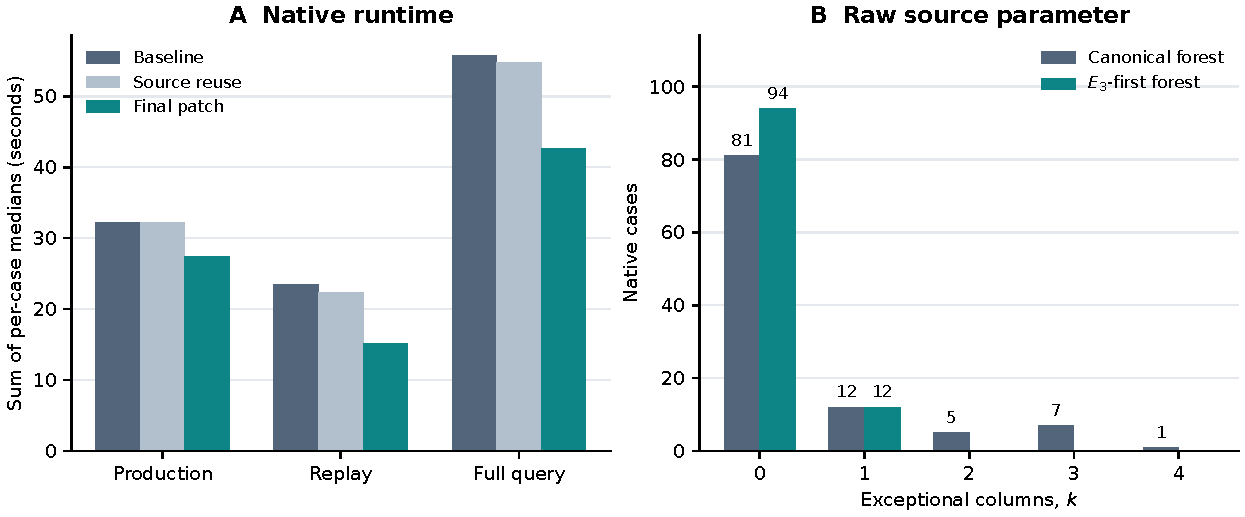
\includegraphics[width=\textwidth]{figures/native_results.pdf}
\caption{Two distinct native results.  Left: complete-query timing of
the behavior-preserving speed patch.  Right: distribution of the raw
exceptional-column count before and after the proved lower-forest parameter
optimization.  The right panel is a source audit, not a timing experiment.}
\label{fig:native-results}
\end{figure}

A separate synthetic experiment isolates endpoint mapping and verifies
exact equality with the preceding naive formula.  It uses equal numbers
of pairings and static gaps, from 64 through 4096, with five paired rounds.
At 4096 pairings the median naive mapper time is 2.3172 seconds and the
median prefix mapper time is 0.004870 seconds.  Their ratio is approximately
476; the median of the five paired ratios is approximately 509.  These
are deliberately labelled mapper-only numbers.  They are not the speedup
of the native recognizer or even of its entire orbit checker.

\begin{figure}[htbp]
\centering
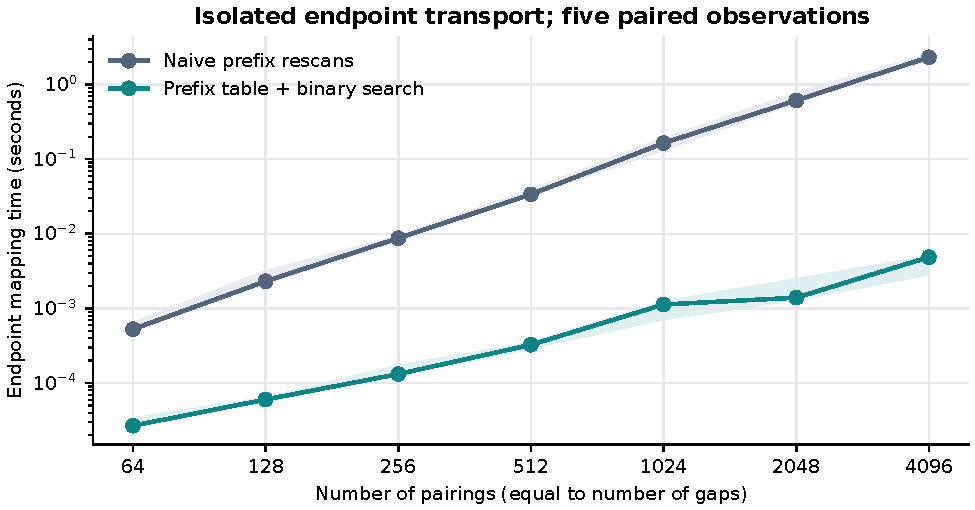
\includegraphics[width=0.83\textwidth]{figures/prefix_scaling.pdf}
\caption{Synthetic endpoint-remapping measurements, with medians and
the range of the five observations.  Both axes are logarithmic.  The theorem
establishes the asymptotic improvement; this experiment isolates the
implementation that realizes it.  Source authentication and other orbit
operations are outside this plot.}
\label{fig:prefix-scaling}
\end{figure}

\subsection{Fresh native parameters and exact finite-core outcomes}

The native exporter checks the raw unsigned occurrence bound on every
one-handle column: total at most three, and at most two for a corner handle.
It also exports the canonical lower forest and a forest attaining
\(\kappa=|E_3|-r_G(E_3)\).  The resulting distributions are:

\begin{center}
\begin{tabular}{lrrrrr}
\toprule
Lower-forest policy & $k=0$ & $k=1$ & $k=2$ & $k=3$ & $k=4$\\
\midrule
Canonical & 81 & 12 & 5 & 7 & 1\\
$E_3$ first & 94 & 12 & 0 & 0 & 0\\
\bottomrule
\end{tabular}
\end{center}

For the canonical matrices, 89 cases have no nonfree special SCC, seven
have one, eight have two, one has three, and one has four.  Their ideal
counts are respectively 1, 2, 4, 8, and 16.  In this raw corpus the surviving
special-SCC orders happen to be antichains, so the ideal refinement does
not further reduce the Boolean state count.  It is a proved structural
improvement whose benefit requires a different order structure.  After
$E_3$-first optimization, the nonfree dimensions are zero in 94 cases,
one in ten, and two in two; the largest ideal count is four.

\begin{table}[htbp]
\centering
\begin{tabular}{lrr}
\toprule
Finite supplied-matrix result & Canonical lower forest & $E_3$ first\\
\midrule
Old two-row solver: success & 81 & 94\\
Old two-row solver: unsupported/inconclusive & 25 & 12\\
Exact history solver: success & 100 & 106\\
Exact history solver: finite infeasibility & 6 & 0\\
Deterministic width solver: success & 100 & 106\\
Randomized ideal solver: success & 100 & 106\\
\bottomrule
\end{tabular}
\caption{The native \emph{raw core} finite problems.  The six unsuccessful
canonical cases yield exact finite negatives in deterministic search and
inconclusive outputs in randomized discovery.  Every positive certificate
passes the separate finite verifier.  These counts are not whole-cut
handlebody counts.}
\label{tab:finite-core}
\end{table}

All 212 finite instances---106 with each lower-forest policy---were also
checked by an independent exhaustive spanning-tree and literal-peeling
oracle.  It enumerated 136 spanning trees for each policy and agreed with
the exact solvers on every instance.  The native dual rank is at most one
in this corpus.  Thus this experiment authenticates a useful native domain
and detects real lower-forest effects, but does not empirically stress the
new theorem at large dual rank.  In particular, all 106 optimized positives
are already found by the deterministic mandatory-group candidate followed
by peeling; none needs a nonzero determinant discovery.  The algebraic
implementation is exercised separately against explicit basis expansions.

The six raw-core rescues are the pilot Fibonacci cases with indices
04, 06, 08 and 10, together with \code{pilot/lst_4_9/0} and
\code{pilot/finite_trefoil/0}.
All 100 prior raw-core successes are preserved by the optimized forest on
this corpus.  That empirical preservation is not asserted as a theorem
for arbitrary inputs.

\subsection{Five additional whole-cut certificates}

A separate, optional producer portfolio first tries the maintained
planner and then two bounded lower-forest policies: $E_3$ first and reverse
edge order.  The finite core proof is replayed, and any completed whole-cut
packet is submitted to the unchanged public whole-cut verifier.  The adapter
uses a private producer-module instance; it does not replace a public
module's planner or alter the certificate schema.

\begin{center}
\begin{tabular}{P{0.57\textwidth}P{0.31\textwidth}}
\toprule
New full-certificate case & Successful alternative\\
\midrule
\code{pilot/fibonacci_lst_04/0} & $E_3$ first\\
\code{pilot/fibonacci_lst_06/0} & $E_3$ first\\
\code{pilot/lst_4_9/0} & $E_3$ first\\
\code{pilot/finite_trefoil/0} & $E_3$ first\\
\code{pachner23_5_8_2/mixed} & Reverse order\\
\bottomrule
\end{tabular}
\end{center}

Each new packet contains the original source, coordinates, and complete
native certificate, with its hash recorded in the audit.  Combining these
five verified positives with the maintained 92 gives 97 complete whole-cut
censuses out of 106.  The original speed patch continues to produce exactly
the original 92 outputs; the coverage increase belongs to the separately
dispatched research portfolio.

The larger Fibonacci cases with indices eight and ten now pass raw core
cancellation but stop at annular attachment.  The finite figure-eight
positive target still stalls in the whole-cut core path in the bounded
search.  These observations identify a geometric continuation problem,
not a reason to relax unsigned cancellation or certificate checks.

A historical Regina oracle audit, tied to this same corpus hash, identifies
eight genuine all-handlebody misses among the original fourteen refusals;
the other six contain at least one non-handlebody piece.  This classification
is explicitly labelled historical in the package; it was not recomputed
as part of the timing run.  The three saved interface obstructions in the
preceding forest report belong to the latter category.  Seeking geometric
moves that preserve the whole cut yet turn all of their components into
handlebodies would therefore be a misguided positive target.  If sphere
capping is intended, it needs its own changed terminal specification and
certificate.

\subsection{Independent finite identities and hostile inputs}

The new unit suite has 15 test methods.  Its exhaustive family covers all
4096 combinations of a binary $3\times2$ matrix and three edge records
chosen from two loops, one eligible edge, and an unavailable edge.  It also
checks 320 weighted instances with wider exceptional columns, 180 small
posets including chains and antichains, all 256 three-variable Boolean
truth tables, resource limits, and certificate/source mutations.

The independent mathematical audit programs add the following checks:

\begin{itemize}
\item 800 matrices, 2836 tree/matrix pairs, and 46\,127 exceptional
  schedules checked against literal peeling;
\item 700 covering instances and 1377 determinant evaluations compared
  with direct common-basis polynomial expansion;
\item 650 Boolean-sieve matrices, 2300 tree/matrix pairs, 8657 activation
  table entries, and 711 determinant-versus-basis comparisons;
\item 1800 random posets on one through nine elements, containing 47\,467
  enumerated ideals, with direct zeta, inverse, maximal-element and filter
  identities checked;
\item 650 further weighted instances, with up to five rows in an
  exceptional support, checked directly against the delivered width and
  randomized implementations and an independent tree/peeling oracle.
\end{itemize}

The focused maintained-runtime regression passes 100 tests, and the separate
portfolio suite passes nine, for 109 distinct implementation tests in total.
These are additional to the 15 finite-solver test methods.  The runtime suite includes
the independent gap arithmetic and source-mutation checks described in
\cref{sec:implementation-prefix}.  Test identities, seeds, commands and raw
reports are included so that a reader can distinguish proof, finite testing,
and a native source-authenticated result.  Finite audits do not replace the
proofs, and passing selected runtime tests does not claim that every test
elsewhere in the large repository was rerun.

\section{From local algorithms to a global complexity argument}
\label{sec:global}

\subsection{An explicit ledger of the remaining obligations}

A local algorithm can be fixed-parameter tractable while the enclosing
recognizer remains exponential.  There are four independent quantities to
control: the cost of producing a legal next surface or move, the number of
states visited, the encoded size of each state, and the cost of resolving
the terminal topology.  A small matrix at one successful cut gives no bound
on the other three quantities.

The reviewed hierarchy preprint supplies a polynomial compressed-cutting
primitive for handle structures of uniform type, polynomial in handle count
and logarithmic extended weight.  It returns the complement of the parallelity
bundle and the bundle topology and attachment data (Theorem 14.4), while
Section 9 separates a step-count analysis from
a full runtime estimate \cite{Lackenby2026}.  This is the appropriate
interface for the present work: geometry must arrive in a compressed,
source-authenticated representation, and its attachment information must
survive every simplification.

\begin{center}
\begin{tabular}{P{0.25\textwidth}P{0.31\textwidth}P{0.33\textwidth}}
\toprule
Obligation & Result available here & Still required globally\\
\midrule
Raw local completion & Exact $J$-state reduction; deterministic width
algorithm & Completeness of the chosen geometric move class at every
needed state.\\
Representation size & No expansion in multiplicity in these finite
operators & Bounds on handles, charts, runs, and integer bit lengths
after all cuts and transports.\\
Hierarchy control & Explicit local cost parameters & A bound on total
states, restarts, and surface-production work.\\
Boundary and bundle data & Existing native verifier; five new accepted
packets & Complete primitive-attachment, puncture, and terminal handling
where current certificates refuse.\\
Randomness & One-sided local witness misses, exact positive replay & A
global error schedule, or a deterministic structural regime.\\
\bottomrule
\end{tabular}
\end{center}

\subsection{A conditional composition bound}

The following accounting statement makes the target testable.  It is a
conditional composition result, not a theorem that the hypotheses hold
for all knot diagrams.

\begin{proposition}[A sufficient deterministic route to quasi-polynomial time]
\label{prop:global-conditional}
Suppose a correct and complete recognition algorithm on $n$-crossing input
diagrams has the following independently established properties:
\begin{enumerate}
\item it visits at most $Q(n)$ states and makes at most polynomially many
  local completion calls per state;
\item each call is equivalent to the finite completion problem of this
  article, with explicit encoded size $N\leq n^b$ for a fixed $b$;
\item all remaining production, transport, and verification work per state
  is bounded by $n^b$ after increasing $b$ if necessary;
\item the implication width of every local call is at most $w(n)$.
\end{enumerate}
If $Q(n)\leq\exp(O((\log n)^a))$ and
$w(n)=O((\log n)^c)$ for fixed $a,c\geq0$, then replacing its finite
completion calls by the deterministic width algorithm gives total time
\[
       \exp\!\left(O\left((\log n)^{\max\{a,c+1,1\}}\right)\right).
\]
In particular it is quasi-polynomial.  The correctness and completeness
assumption includes all geometric and terminal decisions, not only the
existence of the local certificates considered here.
\end{proposition}
\begin{proof}
For $w>0$, the ideal bound gives $J\leq(d+1)^w\leq(N+1)^w$.
The deterministic width algorithm therefore costs $N^{O(w+1)}$ per call.
For $w=0$ it is polynomial as well.  Substituting $N\leq n^b$ gives
\(\exp(O((w(n)+1)\log n))\).  Multiplying by the permitted number of
states and calls and adding the other work yields the displayed bound.
Because each local algorithm solves exactly the specified finite problem,
this replacement does not alter an independently proved global correctness
argument.
\end{proof}

The randomized alternative replaces the local factor by
$2^d\poly(N)$, or more precisely $J\poly(N)$.  With a known upper bound
on the number of relevant calls, distribute a desired total miss allowance
$\varepsilon$ among them and repeat independent identity tests accordingly.
A union bound controls the probability of any required local witness being
missed, provided all other completeness obligations are met.  A zero test
still cannot be treated as a deterministic negative certificate.

For example, polynomial state size and $d=O(\log n)$ give a polynomial
randomized local cost.  Polynomial state size and $w=O(\log n)$ give a
deterministic local cost $\exp(O((\log n)^2))$.  If a hierarchy visits
$\exp(O((\log n)^3))$ states, the total bound remains quasi-polynomial
but has the larger exponent.  This explains why an article must specify
whether it controls local work, the state count, or both.

The bound $k\leq2T$ for a raw core with $T$ tetrahedra is insufficient on
its own: $8^{2T}$ is exponential in $T$.  Nor does observing
$\kappa\leq1$ on 106 inputs establish such a bound on an infinite class.
The useful advance is that there are now precise quantities---$\kappa$,
$d$, $J$, $w$, and $q$---for a global geometric theorem to control.

\section{Proposed research program}
\label{sec:research}

The next projects should have a definite theorem, failure example, or
replayable artifact as their output.  The order below emphasizes the two
current positive gaps in annular attachment, then the structural questions
most directly connected to asymptotic complexity.

\subsection{Geometric continuation and choice of lower forest}

\paragraph{1. Complete the two newly exposed Fibonacci attachment cases.}
The index-eight and index-ten Fibonacci cuts now admit raw core
cancellation under the optimized lower forest, yet their annular interface
stage refuses.  Export the exact remaining annular curves, the lower-forest
basis, and all source endpoint maps.  Determine whether a verified change
of meridian system makes the attachment primitive in the required geometric
sense.  A useful result is a family theorem with a compressed construction,
not just two extra successes.  The deliverable should be a source-bound
move sequence followed by an unchanged terminal check, together with a
bound in layer count and coordinate bit length.

\paragraph{2. Optimize lower forests for completion, not only for $k$.}
The graphic-nullity formula solves the parameter objective exactly, but
minimizing that objective need not preserve a successful attaching pattern.
Study the joint choice of lower and top forests.  First search for an
explicit native example where every minimum-$k$ lower forest fails but
another lower forest succeeds.  If such examples exist, identify a secondary
objective or a bounded family of exchanges that preserves completeness.
If they do not occur in a well-defined native subclass, prove the exchange
property.  The reverse-order rescue of the Pachner case already shows why
a single numerical score should not silently replace a portfolio.

\paragraph{3. Authenticate geometric tightening and handle slides.}
Actual unsigned occurrences can exceed the algebraic obstruction after
curves are tightened or the meridian system changes.  Signed exponent sums,
gcd tests, or free-group simplification alone do not provide the geometric
disc required by the current certificate.  Develop a compiler for an
embedded boundary-curve isotopy or a geometrically realized handle slide,
with certified endpoint transport and intersection counts.  Existing
polynomial compressed-curve algorithms supply relevant primitives
\cite{LackenbyCurves2026}; the open work is their integration with this
marked source representation and simultaneous annular attachments.
The first milestone is a checker for one move, including its inverse and
the preservation of boundary pattern and orientability.

\paragraph{4. Specify punctured-handlebody terminals separately.}
Six original refusals contain non-handlebody pieces according to the
historical oracle.  Some applications may instead want a handlebody after
certified sphere capping.  Define that terminal class explicitly, including
which boundary spheres are capped and how the original component is
recovered.  A new puncture certificate should not be accepted as an ordinary
handlebody certificate.  This project can turn otherwise misleading
``misses'' into a useful terminal specification while preserving the
logical meaning of the existing genus census.

\subsection{Sharper structural parameters and exact algorithms}

\paragraph{5. Exploit native cycle compatibility of triple supports.}
The current theorem permits arbitrary exceptional supports.  Source
boundary compatibility imposes additional mod-two cycle conditions in the
dual graph, as audited in the preceding normalization report
\cite{IncomingForests2026}.  A three-edge even subgraph has very restricted
forms, involving triangles, parallel edges, and loops.  Determine whether
these constraints give a stronger exchange theorem, a smaller effective
parameter, or a polynomial class beyond support two.  The target is an
exact reduction respecting actual unsigned entries; parity can constrain
the search but cannot substitute for a unit crossing.  Any hardness
construction used to delimit this problem must satisfy the native source
constraints before being called a topological hardness result.

\paragraph{6. Saturate unary consequences before building the poset.}
Forward chaining from one row may imply another through several nonlinear
rules.  Such a unary logical consequence is safe to add as an ordinary
implication if its derivation is retained.  Investigate whether repeatedly
adding these consequences substantially collapses the special-SCC poset,
and prove the exact correspondence with the original closure semantics.
The obvious polynomial preprocessing tries closure from each row.  The
interesting questions are whether a smaller set of representatives suffices,
how much $J$ or $w$ can decrease, and whether native zero patterns impose
a uniform bound on the saturated width.  The positive checker can continue
to replay the final tree and pivots in the original matrix.

\paragraph{7. Determine the best exact route when $q$, $w$, and $d$ differ.}
The present alternatives have costs $J\poly(N)$ with one-sided randomness,
$J(m+1)^w\poly(N)$ deterministically, and $2^qJ\poly(N)$ by exact counting.
Implement the Kirchhoff alternative with fraction-free or certified modular
determinants, then compare these regimes using source-derived parameters.
Seek a deterministic $2^{O(d)}\poly(N)$ algorithm when $q$ is large.
The signed common-basis polynomial is the concrete difficulty; a positivity
argument for a different polynomial must prove that it has exactly the
required support.  General nonnegative-polynomial detection results are
relevant context, but do not directly apply to the mixed-sign common-basis
enumerator \cite{BrandKorchemnaSkotnica2023}.

\paragraph{8. Replace large explicit ideal tables when the frontier is small.}
A poset can have many ideals even when a particular elimination ordering
has a small active frontier.  Study a decision diagram or a dynamic program
that compiles the activation function and ideal constraints together.
Specify exactly what boundary information must be retained so that a tree
outside the processed region is represented faithfully.  It is not enough
to compress the Boolean function if the graphic common-basis constraints
lose their dependence across the boundary.  A useful theorem would express
time in an explicitly defined width of the combined dependency and graphic
structure, with an independent witness extractor.

\subsection{Verification, representation size, and the hierarchy}

\paragraph{9. Produce portable negative finite certificates.}
The deterministic search can exhaust its finite space, but most of its
negative outputs currently have no exported proof object.  Develop a
certificate that an independent checker can validate without trusting the
search program.  Possible starting points are per-state graphic rank
obstructions, a shared acyclic proof of all failed representative choices,
or exact Kirchhoff filtered counts in the small-$q$ regime.  The certificate
must remain bound to the original graph and matrix, and its verification
cost and size should be included in the parameter bound.  Randomized zero
evaluations are insufficient.

\paragraph{10. Improve the remaining compressed transport costs.}
The prefix theorem removes repeated gap sums, but the measured runtime
still includes weight-run overlays, translations, reflection folds,
selector restoration, and repeated trace traversals.  Profile these after
the current patch.  Investigate sorted batched endpoint transport and
interval-run composition, with explicit bit bounds and retained/deleted
endpoint conventions.  A proposed improvement should preserve independently
authenticated gap lists and demonstrate a gain on complete native replay.
The corpus's $2^{16384}$ coordinate scale is a useful check that a convenient
array representation has not introduced point expansion.

\paragraph{11. Build native stress families for the actual new parameters.}
The present raw corpus has dual rank at most one and very small ideal
counts.  Create triangulated source families with increasing dual rank,
controlled exceptional-column cycles, nontrivial implication chains, and
large binary coordinates.  Report $T$, row count, dual rank, $k$, $\kappa$,
$d$, $J$, $w$, $q$, certificate size, and replay time.  Keep abstract
graph/matrix generators separately labelled: they are excellent logical
tests but do not establish realizability by a triangulated source.
Prioritize families that distinguish an exponential number of activation
masks from a polynomial number of ideals.

\paragraph{12. Prove a hierarchy-wide complexity budget.}
Track the number of active nonparallel handles, boundary-pattern records,
interval runs, restart events, and coordinate bit lengths throughout a
complete hierarchy implementation.  Seek an amortized invariant bounding
both the number of visited states and the maximum local ideal complexity.
A decrease in handle count alone is insufficient if a restart duplicates
many states or an attachment representation grows too quickly.  The desired
deliverable is a theorem supplying the hypotheses of
\cref{prop:global-conditional}, or a counterexample showing which proposed
potential fails.  This is the central remaining bridge from the proved
local operators to Lackenby's announced asymptotic target.

\subsection{Recommended next integration checkpoint}

The behavior-preserving speed patch is ready for ordinary code review and
the repository's usual integration gates.  The lower-forest portfolio is
separate and can be reviewed with its five full packets and shared resource
limits.  The exceptional-row solvers should enter as research operators
with measured dispatch parameters, explicit state/work limits, and the
unchanged finite verifier.  Their source adapter must carry all lower-forest
and attachment provenance before they are used as native geometric claims.

For the next research iteration, the highest-value concrete target is the
source-authenticated annular continuation of the two larger Fibonacci
examples.  In parallel, the structural priority is to test and then prove
a bound on implication width after geometric simplification.  Those tasks
would connect the native coverage improvement and the new deterministic
complexity theorem at an interface where both can be checked precisely.

\appendix
\section{Reproduction, integration, and the certificate boundary}
\label{sec:reproducibility}

\subsection{Package structure and source pin}

The package is intended for review before incorporation into ProveIt.
The LaTeX article, source fragments, vector figures, executable algorithms,
independent audits, raw measurements, source-bound packets and patches
are all included.  The root \code{README.md} gives exact commands and
the recommended patch order.  \code{PROVENANCE.json} identifies the
repository pin, the five inspected incoming archives, and their hashes;
\code{MANIFEST.sha256} inventories the delivered files.

The main LaTeX source is
\code{article/exceptional_rows_and_certificate_replay.tex}.
Compile from its directory with:
\begin{lstlisting}
latexmk -pdf -interaction=nonstopmode -halt-on-error \
  exceptional_rows_and_certificate_replay.tex
\end{lstlisting}
The source uses standard LaTeX packages.  Its figures are included as
vector PDFs; rebuilding them uses Python, NumPy, and Matplotlib.  The
finite forest solvers and their independent checker use only Python's
standard library.  Native reproductions use the dependencies of the
maintained ProveIt fast package.

\subsection{Finite problem schema and available algorithms}

The finite input is a JSON object with exactly four fields:
\begin{lstlisting}
{
  "vertices": 2,
  "columns": 2,
  "edges": [[0, 1], [0, 1], [0, 0]],
  "rows": [[[0, 1], [1, 1]], [[0, 1], [1, 2]], [[0, 1]]]
}
\end{lstlisting}
Row $i$ has edge record $i$.  A missing eligible edge is encoded by
\code{null}; loops are also ineligible.  Each sparse row lists distinct
column indices and strictly positive integer counts.  Booleans are not
accepted as integers.  Root vertex zero is distinguished.  Empty matrices,
isolated source vertices, large integer labels and multiplicities, repeated
edges and invalid records have explicit validation behavior.

\begin{center}
\begin{tabular}{P{0.31\textwidth}P{0.32\textwidth}P{0.26\textwidth}}
\toprule
Entry point & Search & Negative convention\\
\midrule
\code{solver.solve} & Exact exceptional schedules, support at most three
for useful columns & Exhaustive \code{NO_FOREST}; limits are inconclusive.\\
\code{solver.solve_randomized} & Reference schedule plus covering sieve
& A randomized zero is inconclusive.\\
\code{nonlinear.solve_boolean} & SCC/ideal determinant sieve, arbitrary
exceptional support & A randomized zero is inconclusive.\\
\code{nonlinear.solve_width} & Exact streamed ideals and minimal-frontier
representatives & Exhaustive \code{NO_FOREST}; limits are inconclusive.\\
\code{base_verify.verify} & Independent tree and original-matrix replay
& Accepts only supported proof objects.\\
\bottomrule
\end{tabular}
\end{center}

Every success carries a tree and complete peel sequence.  The public
discovery functions construct these by exact integer operations; callers
that rely on the result must invoke the supplied independent checker.
The tests and audit programs do so for every reported positive.  They do
not regard a discovery program's own assertions as independent verification.

The implementation stores ideal coefficients as integers.  The formula
\[
 c(A)=\sum_{S\subseteq\max(A)}(-1)^{|S|}g(A\setminus S)
\]
bounds their
absolute values by $2^d$, so the coefficient storage is
$J\poly(N)$ bits.  The sharper $O(2^d\log N)$ theoretical table bound
in the Boolean theorem uses residues modulo the prime; the delivered
integer tables still satisfy the stated $J\poly(N)$ ideal bound.

The fixed default prime is $2^{61}-1$.  The implementation checks primality
within an explicit 64-bit domain and requires the chosen prime to exceed
twice the number of eligible edges when constructing the determinant
sieve.  Thus the prime characteristic exceeds every copy count and provides
distinct Vandermonde labels.  For arbitrary asymptotic input sizes, the
mathematical algorithm chooses a prime in a polynomial interval rather
than relying on this fixed implementation constant.

An omitted random seed uses uniform system randomness.  A supplied seed
makes experiments reproducible; a probability bound is justified by the
uniform independent sampling model, not by one particular pseudorandom
seed.  Once an evaluation is nonzero, extraction uses no further randomness.
Resource caps return \code{INCONCLUSIVE}.  Most exhaustive deterministic
negative answers do not yet carry a portable negative proof, as their
\code{certificate} field and evidence string make explicit.

\subsection{A minimal example that needs exceptional propagation}

The JSON example above has rows $a,b,c$ and unsigned matrix
\[
        A=\begin{pmatrix}1&1\\1&2\\1&0\end{pmatrix}.
\]
The first column is exceptional.  The second gives the ordinary implication
$b\to a$.  Rows $a$ and $b$ are parallel eligible edges; $c$ is a root loop.
Deleting $a$ as the spanning tree leaves two owners of the triple column
and a coefficient two in the other column, so peeling stalls.  Deleting
$b$ instead allows $a$ to peel on column one and then $c$ on column zero.
The certificate is the tree \([1]\) and peel sequence \([(0,1),(2,0)]\).

The special-row poset has relation $b\prec a$ and isolated element $c$.
It has six ideals rather than eight Boolean subsets.  This example makes
the conjunction and order-ideal reduction visible in a small input; the
general results are justified by the proofs and the separately authenticated
native experiments, not by the example alone.

\subsection{Counterexamples that constrain the algebraic implementation}

\paragraph{Future heads cannot satisfy their own premises.}
Take a one-vertex dual graph, so no row can be deleted by a tree, and the
matrix
\[
        \begin{pmatrix}1&2&2\\1&1&0\\1&0&1\end{pmatrix}.
\]
The first column is a triple; the ordinary implications are $a\to b$ and
$a\to c$.  There is no initial seed and no legal first peel.  A proposed
exceptional head $a$ cannot be used in advance to justify its prerequisites
$b,c$.  This rejects the tempting but invalid replacement of the prefix
head set $H_{i-1}$ by the final head set in the schedule reduction.

\paragraph{Different copies need different variables.}
Consider a rank-two star with two edges $e_1,e_2$, both in one mandatory
group.  Its copied common-basis polynomial has the form
\[
     z_{1,\mathrm{rep}}z_{2,\mathrm{fill}}
       -z_{1,\mathrm{fill}}z_{2,\mathrm{rep}}.
\]
There is a valid spanning tree.  Identifying representative and filler
variables for each original edge makes the polynomial identically zero.
The independent variable for each copy is therefore part of the theorem,
not an implementation convenience.

\paragraph{One deletion scan is insufficient over a field.}
For three parallel edges in rank one, take
$Q=x_1+x_2+x_3$ over $\mathbb F_7$ and evaluate at $(1,1,6)$.
The total is one.  Removing the first or second variable yields zero;
removing the third leaves two.  A single scan can therefore stop with two
variables.  A second scan extracts one.  The repeated-scan implementation
tests this exact regression.

\paragraph{Field cardinality does not replace characteristic.}
Over any characteristic-two extension, the same polynomial evaluated at
$(1,1,1)$ is nonzero, while every one-variable deletion is zero.  Euler's
identity then only gives $3\equiv1\pmod2$.  Arbitrarily large extension
fields do not fix this example.  The extraction lemma needs characteristic
greater than the initial number of variables.

\paragraph{Inverse ideal transforms need reverse topological order.}
For a chain $a\prec b$, the coefficient of its full ideal is
$g(\{a,b\})-g(\{a\})$.  Processing $a$ before $b$ in the subtraction
transform introduces an erroneous $g(\varnothing)$ term.  A regression
also labels ordinary rows in the reverse of their reachability order,
ensuring that sorting row identifiers cannot masquerade as topological
sorting.

\subsection{Evidence levels and implementation status}

\begin{longtable}{P{0.29\textwidth}P{0.28\textwidth}P{0.31\textwidth}}
\toprule
Claim & Evidence delivered & Boundary\\
\midrule
\endhead
Finite schedule/ideal/width theorems & Mathematical proofs; independent
finite audits; executable solvers & Supplied rooted graph and unsigned
matrix; not a general handlebody theorem.\\
Kirchhoff exact counting & Complete proof with bit bound & Not a separate
delivered optimized solver.\\
Native raw arity and optimal $k$ & Local source proof; fresh source/reference
equality checks & Before arbitrary bundle augmentation or slides.\\
Prefix contraction & Exact quotient/inverse proof; independent finite tests
& Endpoint substep, not the whole orbit algorithm.\\
23.48\% full-query reduction & Five paired rounds; complete returned-object
equality on 106 cases & Recorded host and workload only.\\
Five new whole-cut positives & Original-source packets; unchanged public
verifier acceptance & Bounded two-policy portfolio, not exhaustive forest
search.\\
Historical oracle split & Prior report and identical corpus hash & Supporting
classification, not a fresh oracle run or the new proof.\\
Global quasi-polynomial recognition & Conditional accounting proposition
and explicit research obligations & Not established in this continuation.\\
\bottomrule
\end{longtable}

The mathematical proofs are conventional written proofs, accompanied by
independent executable checks.  They have not been formalized in Lean.
Natural formalization targets are the closure equivalence, source-SCC
criterion, ideal inversion identity, and fixed-evaluation extraction lemma;
each has a small explicit interface independent of three-manifold geometry.

\begin{thebibliography}{99}
\raggedright
% Input inside an existing thebibliography environment.
% These entries mirror verified_standard_references.bib.

\bibitem{Rado1942}
R.~Rado, A theorem on independence relations,
\emph{The Quarterly Journal of Mathematics} \textbf{os-13}(1) (1942),
83--89. \url{https://doi.org/10.1093/qmath/os-13.1.83}.

\bibitem{Edmonds1979}
J.~Edmonds, Matroid intersection, in P.~L.~Hammer, E.~L.~Johnson,
and B.~H.~Korte (eds.), \emph{Discrete Optimization I},
Annals of Discrete Mathematics \textbf{4}, North-Holland, Amsterdam,
1979, pp.~39--49. \url{https://doi.org/10.1016/S0167-5060(08)70817-3}.

\bibitem{Lawler1975}
E.~L.~Lawler, Matroid intersection algorithms,
\emph{Mathematical Programming} \textbf{9} (1975), 31--56.
\url{https://doi.org/10.1007/BF01681329}.

\bibitem{Harvey2009}
N.~J.~A.~Harvey, Algebraic algorithms for matching and matroid problems,
\emph{SIAM Journal on Computing} \textbf{39}(2) (2009), 679--702.
\url{https://doi.org/10.1137/070684008}.

\bibitem{EibenKoanaWahlstrom2025}
E.~Eiben, T.~Koana, and M.~Wahlstr\"om, Determinantal sieving,
\emph{TheoretiCS} \textbf{4} (2025), Article~21.
\url{https://doi.org/10.46298/theoretics.25.21}.

\bibitem{FastZeta2012}
A.~Bj\"orklund, T.~Husfeldt, P.~Kaski, M.~Koivisto, J.~Nederlof,
and P.~Parviainen, Fast zeta transforms for lattices with few irreducibles,
in \emph{Proceedings of the Twenty-Third Annual ACM-SIAM Symposium
on Discrete Algorithms}, SIAM, 2012, pp.~1436--1444.
\url{https://doi.org/10.1137/1.9781611973099.113}.

\bibitem{KaskiKohonenWesterback2016}
P.~Kaski, J.~Kohonen, and T.~Westerb\"ack, Fast M\"obius inversion
in semimodular lattices and ER-labelable posets,
\emph{The Electronic Journal of Combinatorics} \textbf{23}(3) (2016),
Paper~P3.26. \url{https://doi.org/10.37236/5998}.

\bibitem{Dilworth1950}
R.~P.~Dilworth, A decomposition theorem for partially ordered sets,
\emph{Annals of Mathematics}, Second Series, \textbf{51}(1) (1950),
161--166. \url{https://doi.org/10.2307/1969503}.

\bibitem{Chaiken1982}
S.~Chaiken, A combinatorial proof of the all minors matrix tree theorem,
\emph{SIAM Journal on Algebraic Discrete Methods} \textbf{3}(3) (1982),
319--329. \url{https://doi.org/10.1137/0603033}.

\bibitem{Bareiss1968}
E.~H.~Bareiss, Sylvester's identity and multistep integer-preserving
Gaussian elimination, \emph{Mathematics of Computation}
\textbf{22}(103) (1968), 565--578.
\url{https://doi.org/10.1090/S0025-5718-1968-0226829-0}.

\bibitem{Schwartz1980}
J.~T.~Schwartz, Fast probabilistic algorithms for verification of
polynomial identities, \emph{Journal of the ACM} \textbf{27}(4)
(1980), 701--717. \url{https://doi.org/10.1145/322217.322225}.

\bibitem{Zippel1979}
R.~Zippel, Probabilistic algorithms for sparse polynomials,
in E.~W.~Ng (ed.), \emph{Symbolic and Algebraic Computation},
Lecture Notes in Computer Science \textbf{72}, Springer, 1979,
pp.~216--226. \url{https://doi.org/10.1007/3-540-09519-5_73}.

\bibitem{Oxford2021}
Mathematical Institute, University of Oxford,
\emph{Marc Lackenby announces a new unknot recognition algorithm that runs
in quasi-polynomial time}, 2021 announcement.
\url{https://www.maths.ox.ac.uk/node/38304}. Accessed 12 October 2026.

\bibitem{LackenbyTalk2021}
M.~Lackenby, \emph{Unknot recognition in quasi-polynomial time},
Oxford seminar handout, 2021, especially slides 7 and 25 (PDF pages 7 and 25).
\url{https://people.maths.ox.ac.uk/lackenby/quasipolynomial-talk-oxford-compressed.pdf}.

\bibitem{Lackenby2026}
M.~Lackenby, \emph{Incompressible surfaces, hierarchies and unknot recognition},
arXiv:2607.23350v1, 25 July 2026.
\url{https://arxiv.org/abs/2607.23350v1}.

\bibitem{LackenbyCurves2026}
M.~Lackenby, Some fast algorithms for curves in surfaces,
\emph{Discrete \& Computational Geometry} \textbf{76} (2026), 539--588.
\url{https://doi.org/10.1007/s00454-026-00845-7}.

\bibitem{BrandKorchemnaSkotnica2023}
C.~Brand, V.~Korchemna, and M.~Skotnica,
Deterministic constrained multilinear detection,
in \emph{48th International Symposium on Mathematical Foundations of
Computer Science (MFCS 2023)}, LIPIcs \textbf{272}, 25:1--25:14.
\url{https://doi.org/10.4230/LIPIcs.MFCS.2023.25}.

\bibitem{Repo2026}
V.~Reshetnikov, \emph{ProveIt: Topology/UnknotRecognition}, repository,
revision \pin, 12 October 2026.
\url{https://github.com/VladimirReshetnikov/ProveIt/tree/c6d0ec8aa0b6308310ab6c081ba29d8bc363ede5/Topology/UnknotRecognition}.

\bibitem{IncomingPositive2026}
ProveIt incoming research package,
\emph{Positive Cancellation}, 12 October 2026,
\code{ProveIt_Positive_Cancellation_2026-10-12.zip} in
\code{docs/incoming} at the pinned revision.
Article, code, and validation records inspected; archive hash in
\code{PROVENANCE.json} of this delivery.

\bibitem{IncomingForests2026}
ProveIt incoming research package,
\emph{Dual Forest Normalization}, 12 October 2026,
\code{ProveIt_Dual_Forest_Normalization_2026-10-12.zip} in
\code{docs/incoming} at the pinned revision.
Article, finite kernels, native adapters, and source-parity audit inspected;
archive hash in \code{PROVENANCE.json} of this delivery.

\end{thebibliography}

\end{document}
